\documentclass[a4paper]{book}
\usepackage{a4wide}
\usepackage{makeidx}
\usepackage{fancyhdr}
\usepackage{graphicx}
\usepackage{multicol}
\usepackage{float}
\usepackage{textcomp}
\usepackage{alltt}
\usepackage{times}
\ifx\pdfoutput\undefined
\usepackage[ps2pdf,
            pagebackref=true,
            colorlinks=true,
            linkcolor=blue
           ]{hyperref}
\usepackage{pspicture}
\else
\usepackage[pdftex,
            pagebackref=true,
            colorlinks=true,
            linkcolor=blue
           ]{hyperref}
\fi
\usepackage{doxygen}
\usepackage{hyperref}
\makeindex
\setcounter{tocdepth}{1}
\renewcommand{\footrulewidth}{0.4pt}
\begin{document}
\begin{titlepage}
\vspace*{7cm}
\begin{center}
{\Large coin Reference Manual}\\
\vspace*{1cm}
{\large Generated by Doxygen 1.4.2}\\
\vspace*{0.5cm}
{\small Thu Jul 28 17:05:20 2005}\\
\end{center}
\end{titlepage}
\clearemptydoublepage
\pagenumbering{roman}
\tableofcontents
\clearemptydoublepage
\pagenumbering{arabic}
\chapter{coin Directory Hierarchy}
\section{Directories}
This directory hierarchy is sorted roughly, but not completely, alphabetically:\begin{DoxyCompactList}
\item \contentsline{section}{src}{\pageref{dir_551893842a8579748e8cac726fc2aaac}}{}
\end{DoxyCompactList}

\chapter{coin Class Index}
\section{coin Class List}
Here are the classes, structs, unions and interfaces with brief descriptions:\begin{CompactList}
\item\contentsline{section}{\hyperlink{structcelW}{cel\-W} }{\pageref{structcelW}}{}
\end{CompactList}

\chapter{coin File Index}
\section{File List}
Here is a list of all files with brief descriptions:\begin{CompactList}
\item\contentsline{section}{\hyperlink{Classes_8c}{Classes.c} }{\pageref{Classes_8c}}{}
\item\contentsline{section}{\hyperlink{Classes_8h}{Classes.h} }{\pageref{Classes_8h}}{}
\item\contentsline{section}{\hyperlink{coin__common_8h}{coin\_\-common.h} }{\pageref{coin__common_8h}}{}
\item\contentsline{section}{\hyperlink{Helpers_8c}{Helpers.c} }{\pageref{Helpers_8c}}{}
\item\contentsline{section}{\hyperlink{Helpers_8h}{Helpers.h} }{\pageref{Helpers_8h}}{}
\item\contentsline{section}{\hyperlink{LinearStatistic_8c}{LinearStatistic.c} }{\pageref{LinearStatistic_8c}}{}
\item\contentsline{section}{\hyperlink{LinearStatistic_8h}{LinearStatistic.h} }{\pageref{LinearStatistic_8h}}{}
\item\contentsline{section}{\hyperlink{StreitbergRoehmel_8c}{StreitbergRoehmel.c} }{\pageref{StreitbergRoehmel_8c}}{}
\item\contentsline{section}{\hyperlink{vandeWiel_8c}{vandeWiel.c} }{\pageref{vandeWiel_8c}}{}
\end{CompactList}

\chapter{coin Directory Documentation}
\hypertarget{dir_000000}{
\section{src/ Directory Reference}
\label{dir_000000}\index{src/ Directory Reference@{src/ Directory Reference}}
}


\begin{figure}[H]
\begin{center}
\leavevmode
\includegraphics[width=45pt]{dir_000000_dep}
\end{center}
\end{figure}
\subsection*{Files}
\begin{CompactItemize}
\item 
file \hyperlink{CI__common_8h}{CI\_\-common.h}
\item 
file \hyperlink{CIstuff_8c}{CIstuff.c}
\item 
file \hyperlink{CIstuff_8d}{CIstuff.d}
\item 
file \hyperlink{CIstuff_8h}{CIstuff.h}
\item 
file \hyperlink{Classes_8c}{Classes.c}
\item 
file \hyperlink{Classes_8d}{Classes.d}
\item 
file \hyperlink{Classes_8h}{Classes.h}
\item 
file \hyperlink{LinearStatistic_8c}{Linear\-Statistic.c}
\item 
file \hyperlink{LinearStatistic_8d}{Linear\-Statistic.d}
\item 
file \hyperlink{LinearStatistic_8h}{Linear\-Statistic.h}
\item 
file \hyperlink{StreitbergRoehmel_8c}{Streitberg\-Roehmel.c}
\item 
file \hyperlink{StreitbergRoehmel_8d}{Streitberg\-Roehmel.d}
\item 
file \hyperlink{vandeWiel_8c}{vande\-Wiel.c}
\item 
file \hyperlink{vandeWiel_8d}{vande\-Wiel.d}
\end{CompactItemize}

\chapter{coin Class Documentation}
\hypertarget{structcelW}{
\section{celW Struct Reference}
\label{structcelW}\index{celW@{celW}}
}
\subsection*{Public Attributes}
\begin{DoxyCompactItemize}
\item 
long \hyperlink{structcelW_a47b173a5f8c56a051237cac49ddbef4f}{length}
\item 
double $\ast$ \hyperlink{structcelW_af8a631c01b9310cf542171f4df975499}{c}
\item 
double $\ast$ \hyperlink{structcelW_ab443b2a7120f170c2c5e8012f4dd86d7}{x}
\end{DoxyCompactItemize}


\subsection{Detailed Description}
The probability distribution for the independent two sample problem.

REFERENCE

M.A. van de Wiel (2001). The split-\/up algorithm: a fast symbolic method for computing p-\/values of rank statistics, Computational Statistics, 16, 519-\/538. 

Definition at line 31 of file vandeWiel.c.



\subsection{Member Data Documentation}
\hypertarget{structcelW_af8a631c01b9310cf542171f4df975499}{
\index{celW@{celW}!c@{c}}
\index{c@{c}!celW@{celW}}
\subsubsection[{c}]{\setlength{\rightskip}{0pt plus 5cm}double$\ast$ {\bf celW::c}}}
\label{structcelW_af8a631c01b9310cf542171f4df975499}


Definition at line 33 of file vandeWiel.c.



Referenced by cumulcoef(), fillcell(), initW(), mirrorW(), mymergesort(), numbersmall(), plus(), and reserveW().

\hypertarget{structcelW_a47b173a5f8c56a051237cac49ddbef4f}{
\index{celW@{celW}!length@{length}}
\index{length@{length}!celW@{celW}}
\subsubsection[{length}]{\setlength{\rightskip}{0pt plus 5cm}long {\bf celW::length}}}
\label{structcelW_a47b173a5f8c56a051237cac49ddbef4f}


Definition at line 32 of file vandeWiel.c.



Referenced by cumulcoef(), fillcell(), initW(), mirrorW(), mult(), mymergesort(), numbersmall(), and plus().

\hypertarget{structcelW_ab443b2a7120f170c2c5e8012f4dd86d7}{
\index{celW@{celW}!x@{x}}
\index{x@{x}!celW@{celW}}
\subsubsection[{x}]{\setlength{\rightskip}{0pt plus 5cm}double$\ast$ {\bf celW::x}}}
\label{structcelW_ab443b2a7120f170c2c5e8012f4dd86d7}


Definition at line 34 of file vandeWiel.c.



Referenced by fillcell(), initW(), mirrorW(), mymergesort(), numbersmall(), plus(), and reserveW().



The documentation for this struct was generated from the following file:\begin{DoxyCompactItemize}
\item 
\hyperlink{vandeWiel_8c}{vandeWiel.c}\end{DoxyCompactItemize}

\chapter{coin File Documentation}
\hypertarget{CI__common_8h}{
\section{CI\_\-common.h File Reference}
\label{CI__common_8h}\index{CI_common.h@{CI\_\-common.h}}
}
{\tt \#include $<$R.h$>$}\par
{\tt \#include $<$Rmath.h$>$}\par
{\tt \#include $<$Rinternals.h$>$}\par
{\tt \#include $<$Rdefines.h$>$}\par
{\tt \#include $<$R\_\-ext/Applic.h$>$}\par
{\tt \#include \char`\"{}Classes.h\char`\"{}}\par
{\tt \#include \char`\"{}Linear\-Statistic.h\char`\"{}}\par
{\tt \#include \char`\"{}CIstuff.h\char`\"{}}\par


Include dependency graph for CI\_\-common.h:\begin{figure}[H]
\begin{center}
\leavevmode
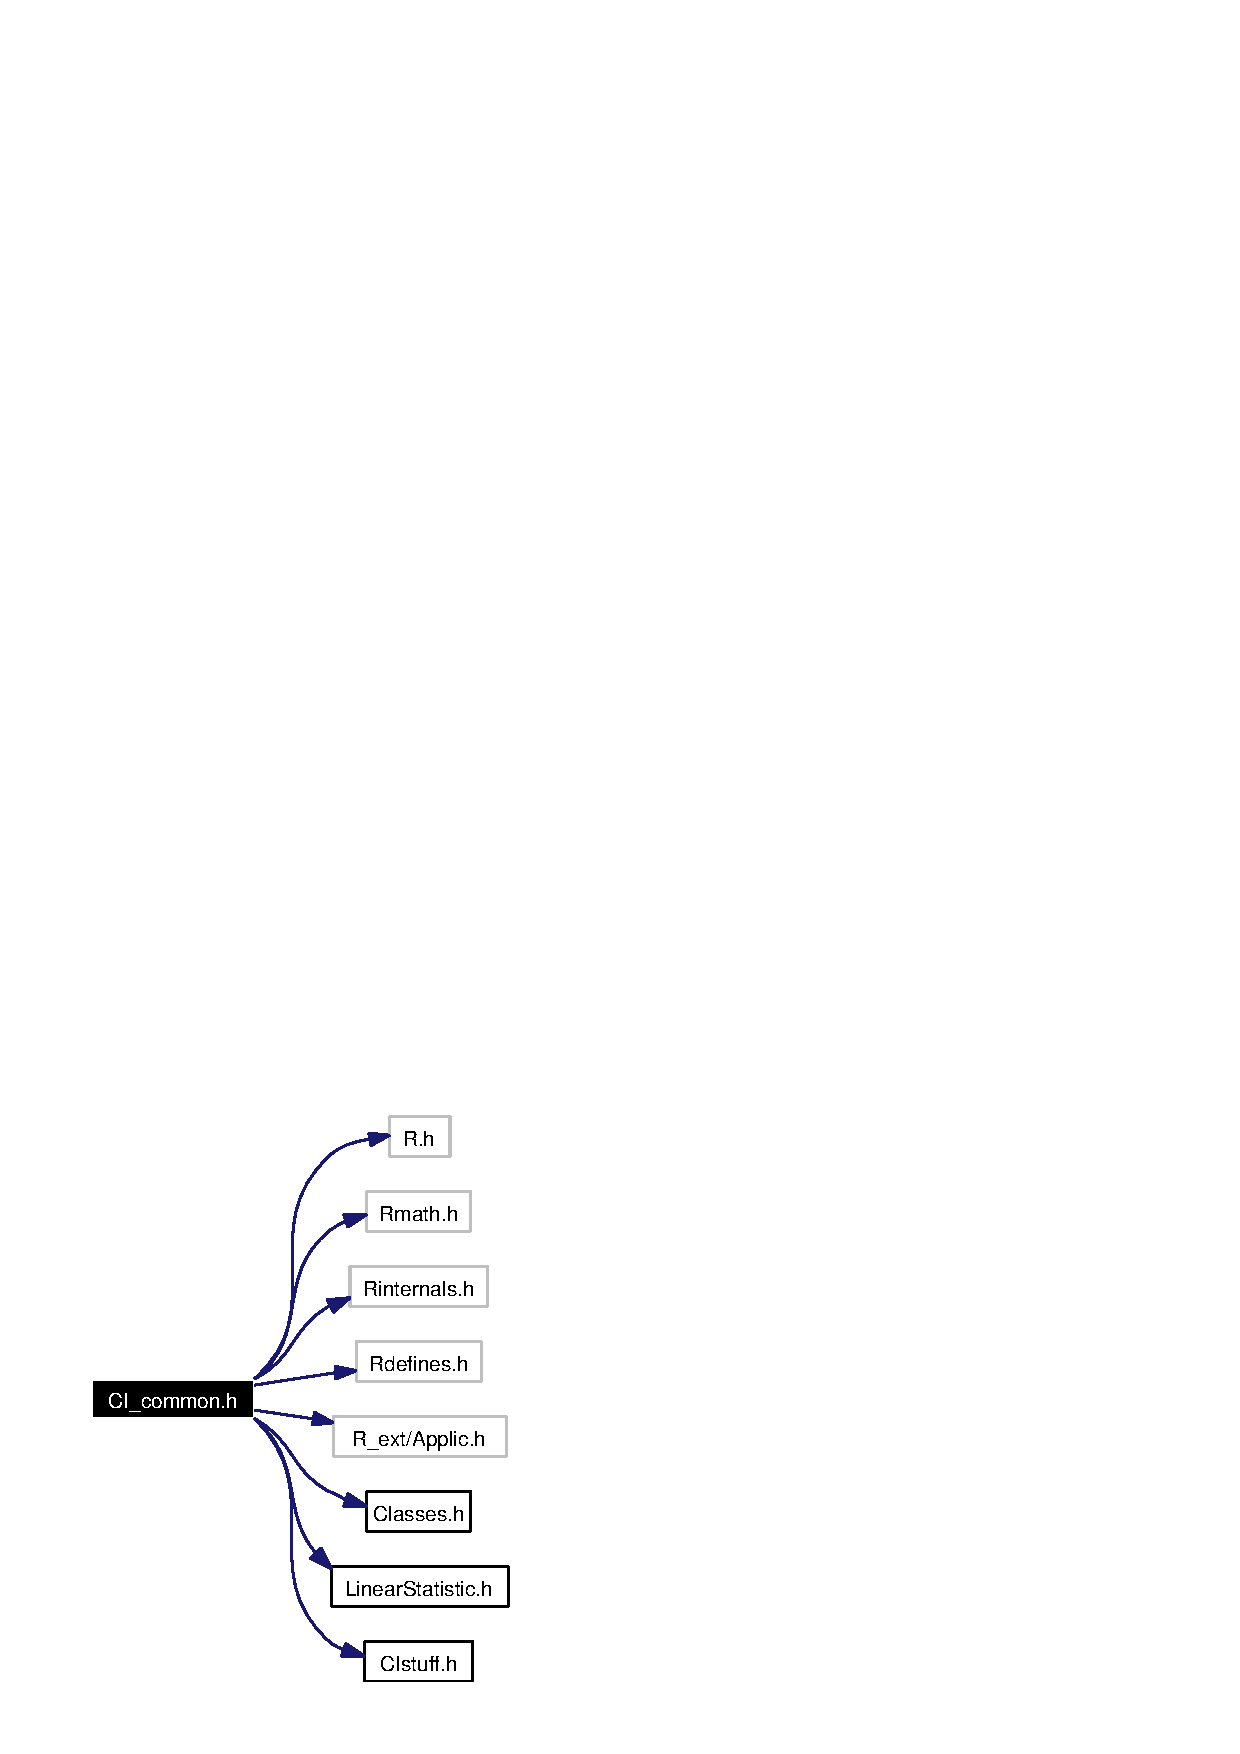
\includegraphics[width=126pt]{CI__common_8h__incl}
\end{center}
\end{figure}


This graph shows which files directly or indirectly include this file:\begin{figure}[H]
\begin{center}
\leavevmode
\includegraphics[width=125pt]{CI__common_8h__dep__incl}
\end{center}
\end{figure}

\hypertarget{CIstuff_8c}{
\section{CIstuff.c File Reference}
\label{CIstuff_8c}\index{CIstuff.c@{CIstuff.c}}
}
{\tt \#include \char`\"{}CI\_\-common.h\char`\"{}}\par


Include dependency graph for CIstuff.c:\begin{figure}[H]
\begin{center}
\leavevmode
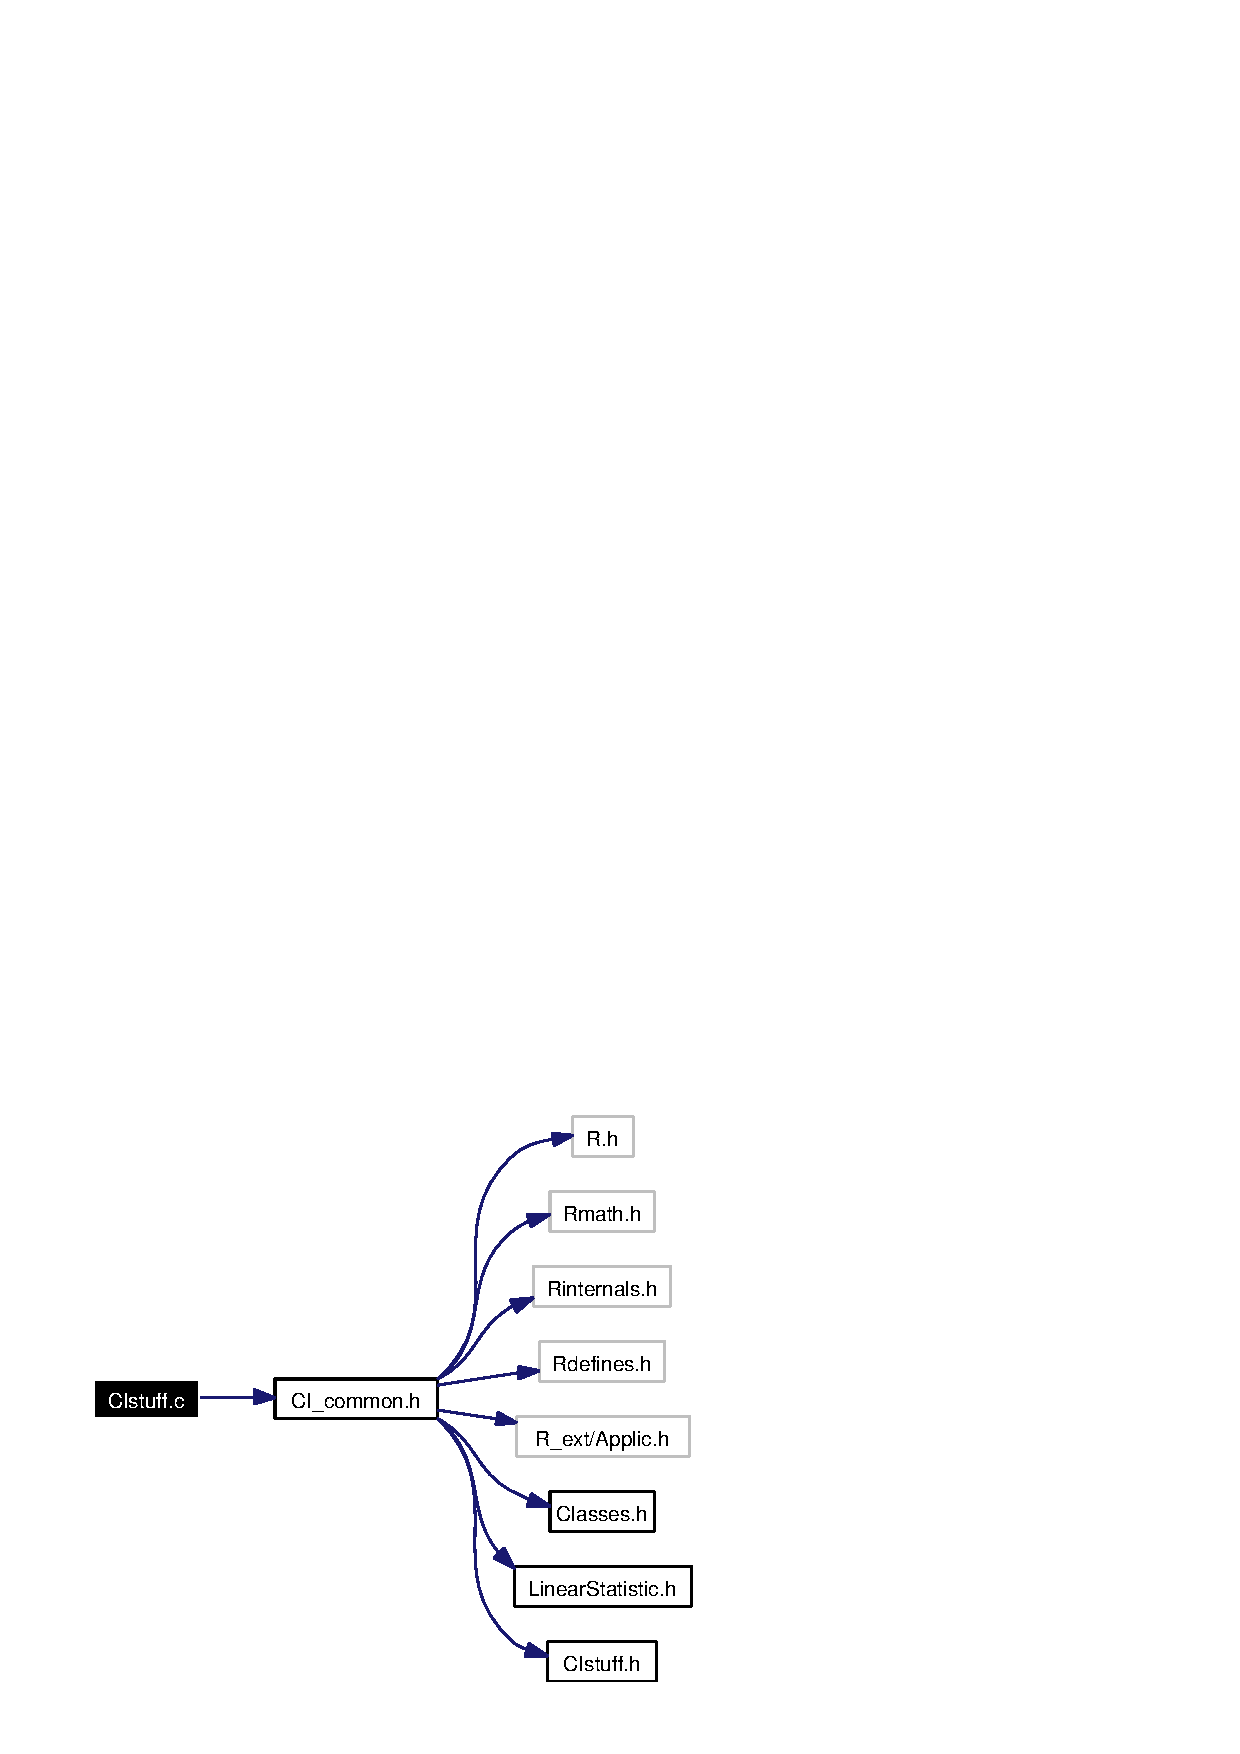
\includegraphics[width=170pt]{CIstuff_8c__incl}
\end{center}
\end{figure}
\subsection*{Functions}
\begin{CompactItemize}
\item 
int \hyperlink{CIstuff_8c_a0}{nrow} (SEXP x)
\item 
int \hyperlink{CIstuff_8c_a1}{ncol} (SEXP x)
\item 
void \hyperlink{CIstuff_8c_a2}{C\_\-Sample\-No\-Replace} (int $\ast$x, int m, int k, int $\ast$ans)
\item 
SEXP \hyperlink{CIstuff_8c_a3}{R\_\-blocksetup} (SEXP block)
\item 
void \hyperlink{CIstuff_8c_a4}{C\_\-blockperm} (SEXP blocksetup, int $\ast$ans)
\item 
SEXP \hyperlink{CIstuff_8c_a5}{R\_\-blockperm} (SEXP block)
\item 
SEXP \hyperlink{CIstuff_8c_a6}{R\_\-Monte\-Carlo\-Independence\-Test} (SEXP x, SEXP y, SEXP block, SEXP B)
\item 
SEXP \hyperlink{CIstuff_8c_a7}{R\_\-maxstattrafo} (SEXP x, SEXP cutpoints)
\end{CompactItemize}


\subsection{Detailed Description}
Some additional functionality for package `coin'

\begin{Desc}
\item[Author:]\begin{Desc}
\item[Author]hothorn \end{Desc}
\end{Desc}
\begin{Desc}
\item[Date:]\begin{Desc}
\item[Date]2005-11-17 13:10:42 +0100 (Thu, 17 Nov 2005) \end{Desc}
\end{Desc}


Definition in file \hyperlink{CIstuff_8c-source}{CIstuff.c}.

\subsection{Function Documentation}
\hypertarget{CIstuff_8c_a4}{
\index{CIstuff.c@{CIstuff.c}!C_blockperm@{C\_\-blockperm}}
\index{C_blockperm@{C\_\-blockperm}!CIstuff.c@{CIstuff.c}}
\subsubsection[C\_\-blockperm]{\setlength{\rightskip}{0pt plus 5cm}void C\_\-blockperm (SEXP {\em blocksetup}, int $\ast$ {\em ans})}}
\label{CIstuff_8c_a4}


Block permutation \begin{Desc}
\item[Parameters:]
\begin{description}
\item[{\em blocksetup}]as computed by `R\_\-blocksetup' \item[{\em ans}]integer vector \end{description}
\end{Desc}


Definition at line 110 of file CIstuff.c.

References C\_\-Sample\-No\-Replace().

Referenced by R\_\-blockperm(), and R\_\-Monte\-Carlo\-Independence\-Test().

Here is the call graph for this function:\begin{figure}[H]
\begin{center}
\leavevmode
\includegraphics[width=139pt]{CIstuff_8c_a4_cgraph}
\end{center}
\end{figure}
\hypertarget{CIstuff_8c_a2}{
\index{CIstuff.c@{CIstuff.c}!C_SampleNoReplace@{C\_\-SampleNoReplace}}
\index{C_SampleNoReplace@{C\_\-SampleNoReplace}!CIstuff.c@{CIstuff.c}}
\subsubsection[C\_\-SampleNoReplace]{\setlength{\rightskip}{0pt plus 5cm}void C\_\-Sample\-No\-Replace (int $\ast$ {\em x}, int {\em m}, int {\em k}, int $\ast$ {\em ans})}}
\label{CIstuff_8c_a2}


compute a permutation of a (random subset of) 0:(m-1) \begin{Desc}
\item[Parameters:]
\begin{description}
\item[{\em x}]an integer vector of length m \item[{\em m}]integer \item[{\em k}]integer \item[{\em ans}]an integer vector of length k \end{description}
\end{Desc}


Definition at line 42 of file CIstuff.c.

Referenced by C\_\-blockperm().\hypertarget{CIstuff_8c_a1}{
\index{CIstuff.c@{CIstuff.c}!ncol@{ncol}}
\index{ncol@{ncol}!CIstuff.c@{CIstuff.c}}
\subsubsection[ncol]{\setlength{\rightskip}{0pt plus 5cm}int ncol (SEXP {\em x})}}
\label{CIstuff_8c_a1}




Definition at line 22 of file CIstuff.c.

Referenced by R\_\-Expect\-Covar\-Influence(), R\_\-Expect\-Covar\-Linear\-Statistic(), R\_\-kronecker(), R\_\-Linear\-Statistic(), R\_\-Monte\-Carlo\-Independence\-Test(), and R\_\-Permuted\-Linear\-Statistic().\hypertarget{CIstuff_8c_a0}{
\index{CIstuff.c@{CIstuff.c}!nrow@{nrow}}
\index{nrow@{nrow}!CIstuff.c@{CIstuff.c}}
\subsubsection[nrow]{\setlength{\rightskip}{0pt plus 5cm}int nrow (SEXP {\em x})}}
\label{CIstuff_8c_a0}




Definition at line 11 of file CIstuff.c.

Referenced by R\_\-Expect\-Covar\-Influence(), R\_\-Expect\-Covar\-Linear\-Statistic(), R\_\-kronecker(), R\_\-Linear\-Statistic(), R\_\-Monte\-Carlo\-Independence\-Test(), and R\_\-Permuted\-Linear\-Statistic().\hypertarget{CIstuff_8c_a5}{
\index{CIstuff.c@{CIstuff.c}!R_blockperm@{R\_\-blockperm}}
\index{R_blockperm@{R\_\-blockperm}!CIstuff.c@{CIstuff.c}}
\subsubsection[R\_\-blockperm]{\setlength{\rightskip}{0pt plus 5cm}SEXP R\_\-blockperm (SEXP {\em block})}}
\label{CIstuff_8c_a5}




Definition at line 139 of file CIstuff.c.

References C\_\-blockperm(), and R\_\-blocksetup().

Here is the call graph for this function:\begin{figure}[H]
\begin{center}
\leavevmode
\includegraphics[width=195pt]{CIstuff_8c_a5_cgraph}
\end{center}
\end{figure}
\hypertarget{CIstuff_8c_a3}{
\index{CIstuff.c@{CIstuff.c}!R_blocksetup@{R\_\-blocksetup}}
\index{R_blocksetup@{R\_\-blocksetup}!CIstuff.c@{CIstuff.c}}
\subsubsection[R\_\-blocksetup]{\setlength{\rightskip}{0pt plus 5cm}SEXP R\_\-blocksetup (SEXP {\em block})}}
\label{CIstuff_8c_a3}




Definition at line 56 of file CIstuff.c.

Referenced by R\_\-blockperm(), and R\_\-Monte\-Carlo\-Independence\-Test().\hypertarget{CIstuff_8c_a7}{
\index{CIstuff.c@{CIstuff.c}!R_maxstattrafo@{R\_\-maxstattrafo}}
\index{R_maxstattrafo@{R\_\-maxstattrafo}!CIstuff.c@{CIstuff.c}}
\subsubsection[R\_\-maxstattrafo]{\setlength{\rightskip}{0pt plus 5cm}SEXP R\_\-maxstattrafo (SEXP {\em x}, SEXP {\em cutpoints})}}
\label{CIstuff_8c_a7}




Definition at line 202 of file CIstuff.c.\hypertarget{CIstuff_8c_a6}{
\index{CIstuff.c@{CIstuff.c}!R_MonteCarloIndependenceTest@{R\_\-MonteCarloIndependenceTest}}
\index{R_MonteCarloIndependenceTest@{R\_\-MonteCarloIndependenceTest}!CIstuff.c@{CIstuff.c}}
\subsubsection[R\_\-MonteCarloIndependenceTest]{\setlength{\rightskip}{0pt plus 5cm}SEXP R\_\-Monte\-Carlo\-Independence\-Test (SEXP {\em x}, SEXP {\em y}, SEXP {\em block}, SEXP {\em B})}}
\label{CIstuff_8c_a6}




Definition at line 152 of file CIstuff.c.

References C\_\-blockperm(), C\_\-Permuted\-Linear\-Statistic(), ncol(), nrow(), and R\_\-blocksetup().

Here is the call graph for this function:\begin{figure}[H]
\begin{center}
\leavevmode
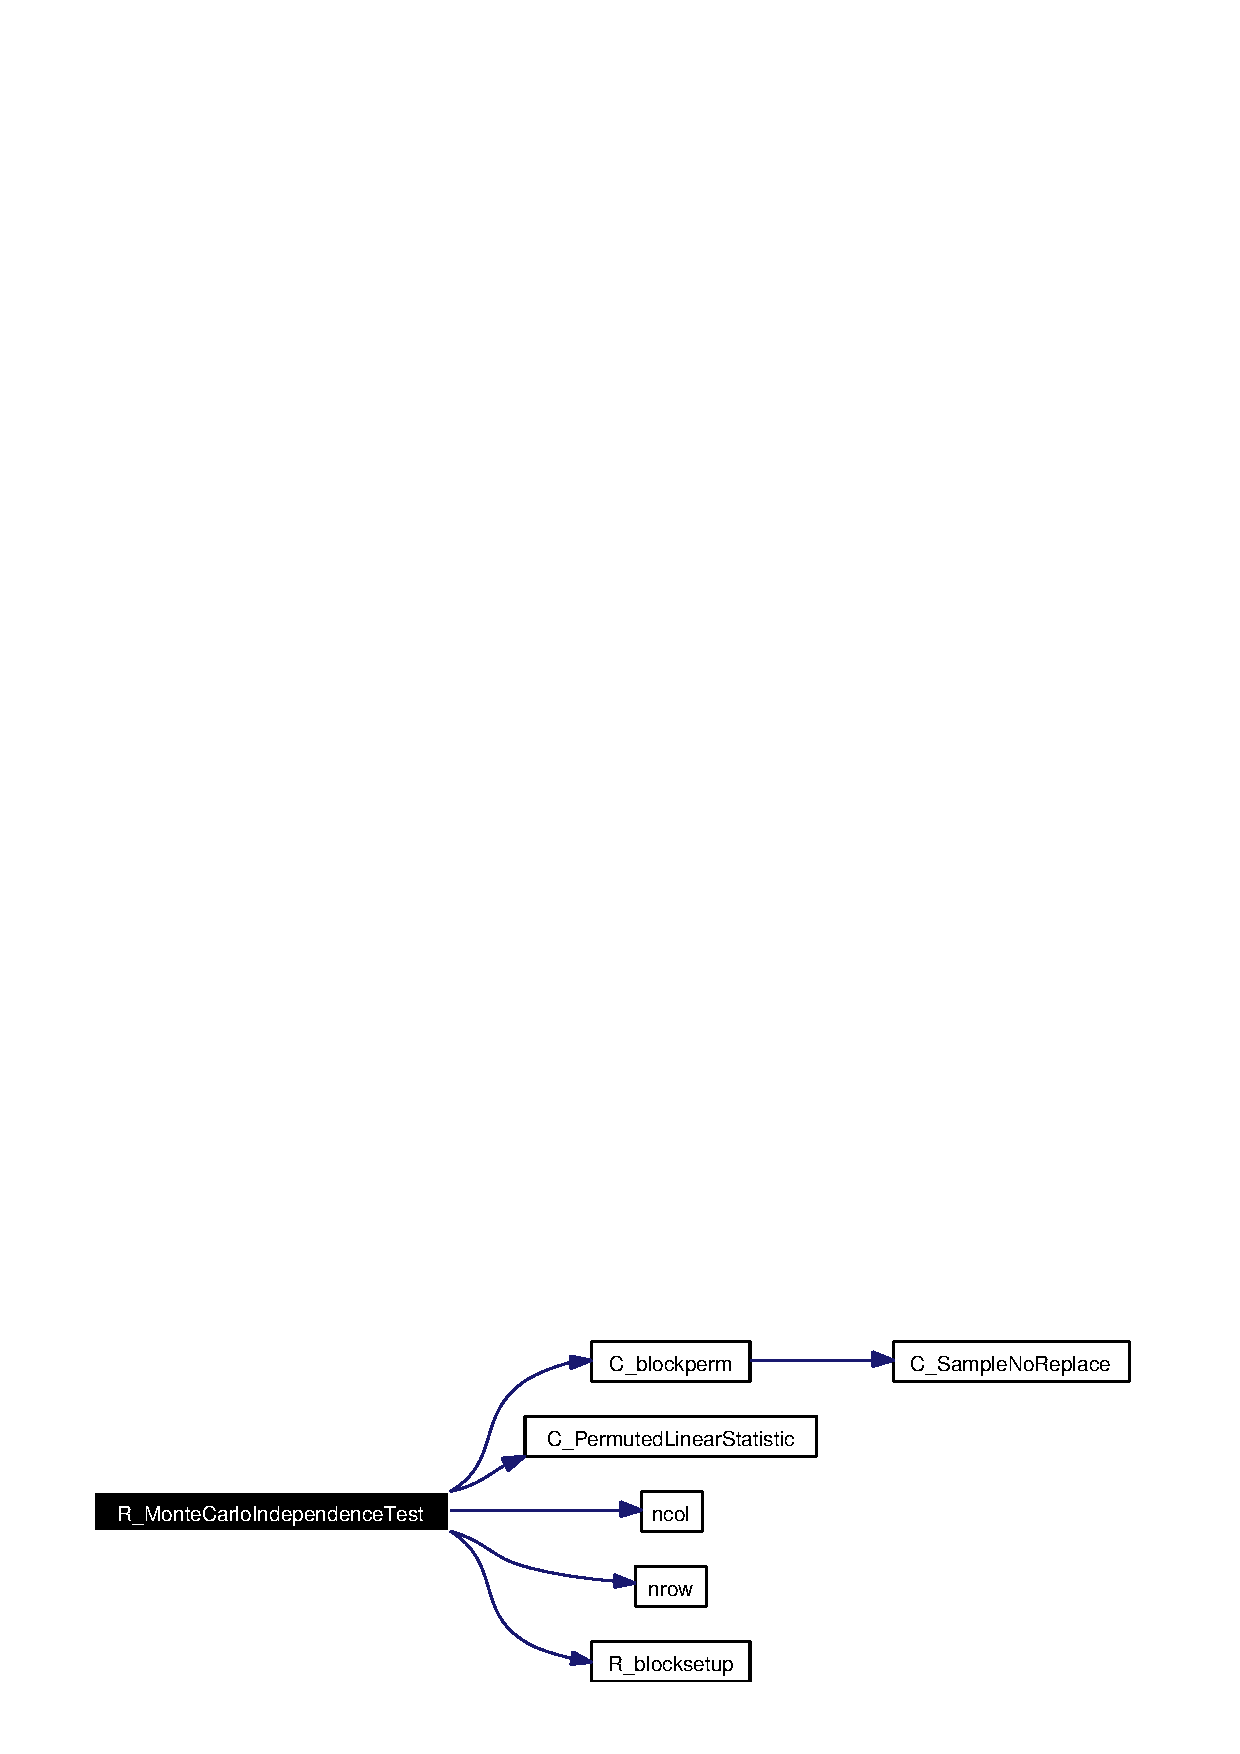
\includegraphics[width=275pt]{CIstuff_8c_a6_cgraph}
\end{center}
\end{figure}

\hypertarget{CIstuff_8d}{
\section{CIstuff.d File Reference}
\label{CIstuff_8d}\index{CIstuff.d@{CIstuff.d}}
}

\hypertarget{CIstuff_8h}{
\section{CIstuff.h File Reference}
\label{CIstuff_8h}\index{CIstuff.h@{CIstuff.h}}
}


This graph shows which files directly or indirectly include this file:\begin{figure}[H]
\begin{center}
\leavevmode
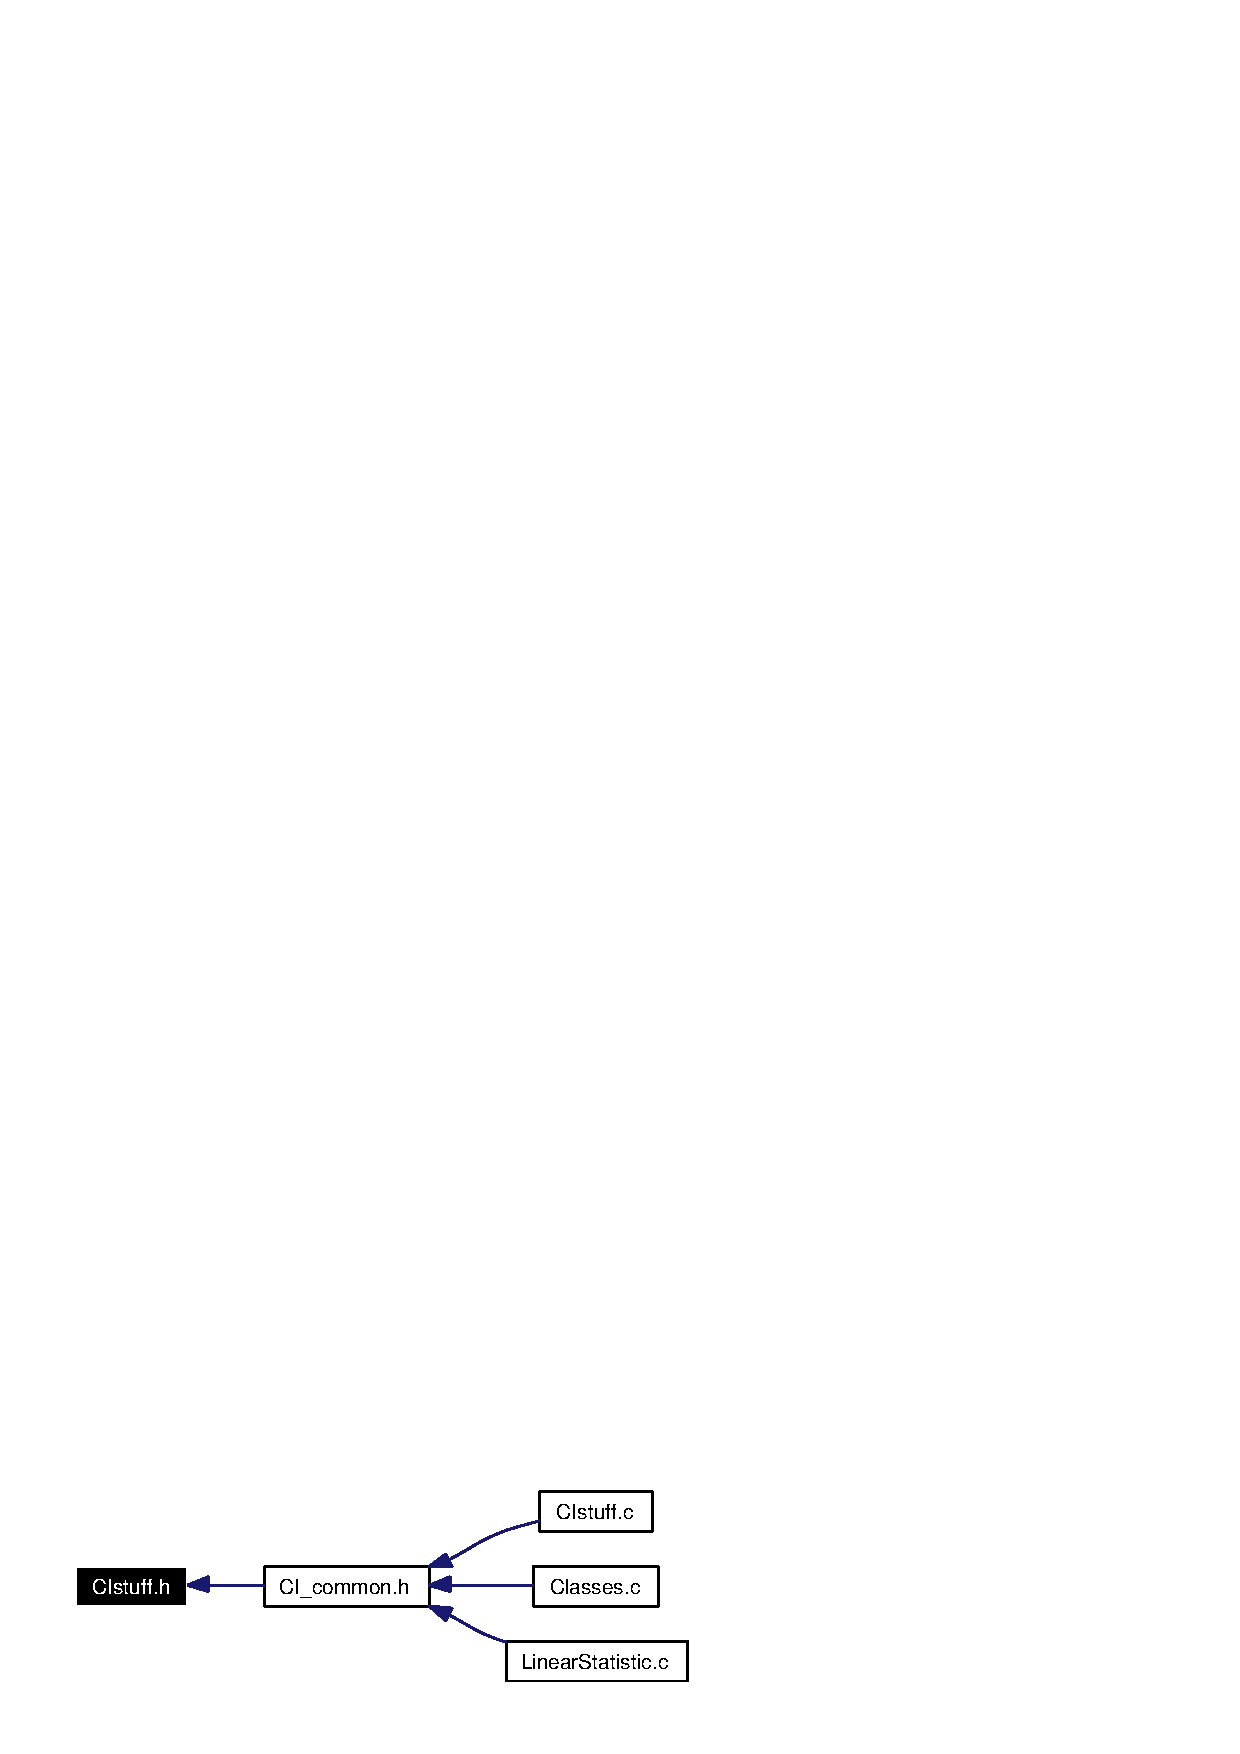
\includegraphics[width=169pt]{CIstuff_8h__dep__incl}
\end{center}
\end{figure}
\subsection*{Functions}
\begin{CompactItemize}
\item 
int \hyperlink{CIstuff_8h_a0}{nrow} (SEXP x)
\item 
int \hyperlink{CIstuff_8h_a1}{ncol} (SEXP x)
\end{CompactItemize}


\subsection{Function Documentation}
\hypertarget{CIstuff_8h_a1}{
\index{CIstuff.h@{CIstuff.h}!ncol@{ncol}}
\index{ncol@{ncol}!CIstuff.h@{CIstuff.h}}
\subsubsection[ncol]{\setlength{\rightskip}{0pt plus 5cm}int ncol (SEXP {\em x})}}
\label{CIstuff_8h_a1}




Definition at line 22 of file CIstuff.c.

Referenced by R\_\-Expect\-Covar\-Influence(), R\_\-Expect\-Covar\-Linear\-Statistic(), R\_\-kronecker(), R\_\-Linear\-Statistic(), R\_\-Monte\-Carlo\-Independence\-Test(), and R\_\-Permuted\-Linear\-Statistic().\hypertarget{CIstuff_8h_a0}{
\index{CIstuff.h@{CIstuff.h}!nrow@{nrow}}
\index{nrow@{nrow}!CIstuff.h@{CIstuff.h}}
\subsubsection[nrow]{\setlength{\rightskip}{0pt plus 5cm}int nrow (SEXP {\em x})}}
\label{CIstuff_8h_a0}




Definition at line 11 of file CIstuff.c.

Referenced by R\_\-Expect\-Covar\-Influence(), R\_\-Expect\-Covar\-Linear\-Statistic(), R\_\-kronecker(), R\_\-Linear\-Statistic(), R\_\-Monte\-Carlo\-Independence\-Test(), and R\_\-Permuted\-Linear\-Statistic().
\hypertarget{Classes_8c}{
\section{Classes.c File Reference}
\label{Classes_8c}\index{Classes.c@{Classes.c}}
}
{\tt \#include \char`\"{}coin\_\-common.h\char`\"{}}\par


Include dependency graph for Classes.c:\begin{figure}[H]
\begin{center}
\leavevmode
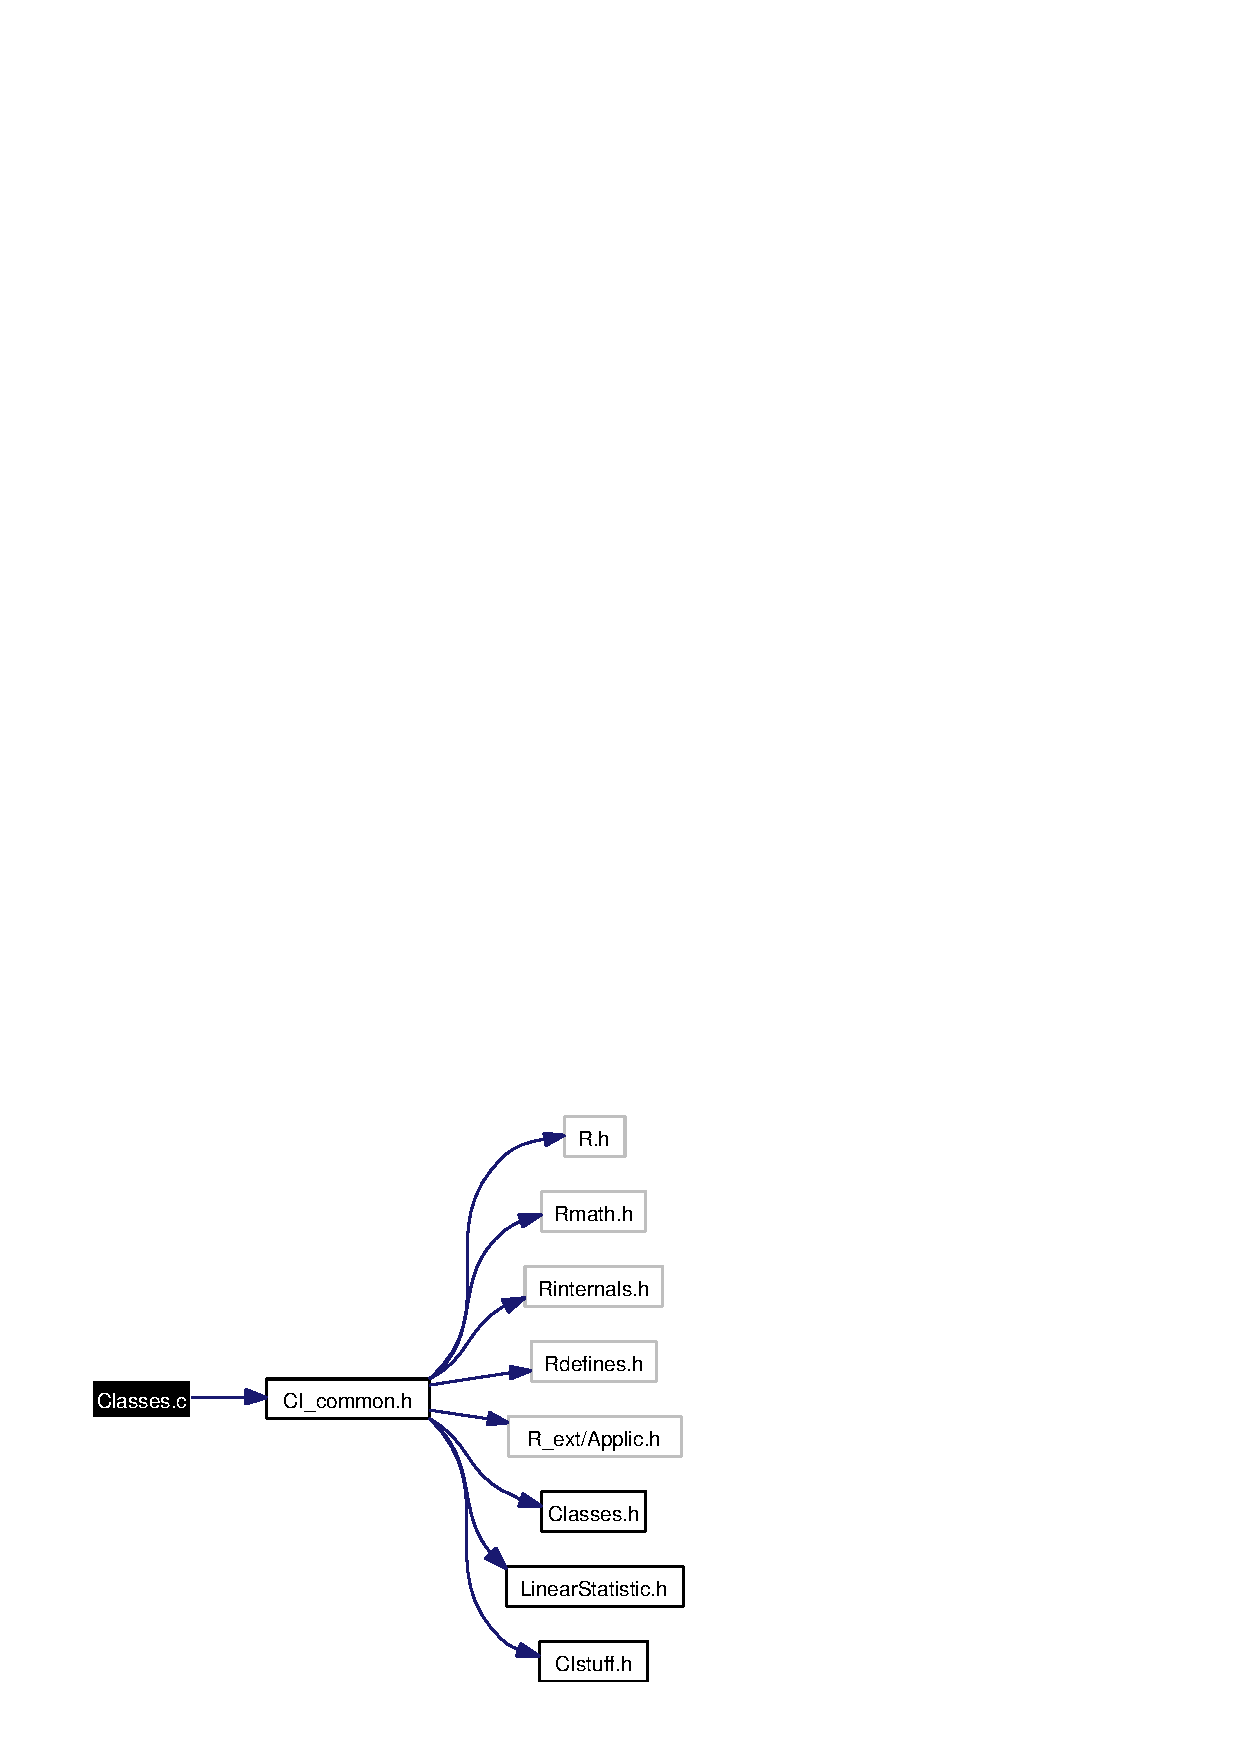
\includegraphics[width=172pt]{Classes_8c__incl}
\end{center}
\end{figure}
\subsection*{Functions}
\begin{CompactItemize}
\item 
SEXP \hyperlink{Classes_8c_5d60a29bf291202b78048a4cd7265a32}{coin\_\-init} (void)
\end{CompactItemize}
\subsection*{Variables}
\begin{CompactItemize}
\item 
SEXP \hyperlink{Classes_8c_bbb9eebf67e5de25bd14a119d80547c8}{coin\_\-expectation\-Sym}
\item 
SEXP \hyperlink{Classes_8c_f9d3f842579c178af113bdaae30eda44}{coin\_\-covariance\-Sym}
\item 
SEXP \hyperlink{Classes_8c_acb7ca69262bcec0b61014b0a152672b}{coin\_\-sumweights\-Sym}
\end{CompactItemize}


\subsection{Detailed Description}
S4 classes

\begin{Desc}
\item[Author:]\begin{Desc}
\item[Author]hothorn \end{Desc}
\end{Desc}
\begin{Desc}
\item[Date:]\begin{Desc}
\item[Date]2007-02-15 09:25:46 +0100 (Thu, 15 Feb 2007) \end{Desc}
\end{Desc}


Definition in file \hyperlink{Classes_8c-source}{Classes.c}.

\subsection{Function Documentation}
\hypertarget{Classes_8c_5d60a29bf291202b78048a4cd7265a32}{
\index{Classes.c@{Classes.c}!coin_init@{coin\_\-init}}
\index{coin_init@{coin\_\-init}!Classes.c@{Classes.c}}
\subsubsection[coin\_\-init]{\setlength{\rightskip}{0pt plus 5cm}SEXP coin\_\-init (void)}}
\label{Classes_8c_5d60a29bf291202b78048a4cd7265a32}




Definition at line 16 of file Classes.c.

References coin\_\-covariance\-Sym, coin\_\-expectation\-Sym, and coin\_\-sumweights\-Sym.

\subsection{Variable Documentation}
\hypertarget{Classes_8c_f9d3f842579c178af113bdaae30eda44}{
\index{Classes.c@{Classes.c}!coin_covarianceSym@{coin\_\-covarianceSym}}
\index{coin_covarianceSym@{coin\_\-covarianceSym}!Classes.c@{Classes.c}}
\subsubsection[coin\_\-covarianceSym]{\setlength{\rightskip}{0pt plus 5cm}SEXP \hyperlink{Classes_8h_f9d3f842579c178af113bdaae30eda44}{coin\_\-covariance\-Sym}}}
\label{Classes_8c_f9d3f842579c178af113bdaae30eda44}




Definition at line 12 of file Classes.c.

Referenced by C\_\-Expect\-Covar\-Influence(), C\_\-Expect\-Covar\-Linear\-Statistic(), coin\_\-init(), R\_\-Expect\-Covar\-Influence(), and R\_\-Expect\-Covar\-Linear\-Statistic().\hypertarget{Classes_8c_bbb9eebf67e5de25bd14a119d80547c8}{
\index{Classes.c@{Classes.c}!coin_expectationSym@{coin\_\-expectationSym}}
\index{coin_expectationSym@{coin\_\-expectationSym}!Classes.c@{Classes.c}}
\subsubsection[coin\_\-expectationSym]{\setlength{\rightskip}{0pt plus 5cm}SEXP \hyperlink{Classes_8h_bbb9eebf67e5de25bd14a119d80547c8}{coin\_\-expectation\-Sym}}}
\label{Classes_8c_bbb9eebf67e5de25bd14a119d80547c8}




Definition at line 12 of file Classes.c.

Referenced by C\_\-Expect\-Covar\-Influence(), C\_\-Expect\-Covar\-Linear\-Statistic(), coin\_\-init(), R\_\-Expect\-Covar\-Influence(), and R\_\-Expect\-Covar\-Linear\-Statistic().\hypertarget{Classes_8c_acb7ca69262bcec0b61014b0a152672b}{
\index{Classes.c@{Classes.c}!coin_sumweightsSym@{coin\_\-sumweightsSym}}
\index{coin_sumweightsSym@{coin\_\-sumweightsSym}!Classes.c@{Classes.c}}
\subsubsection[coin\_\-sumweightsSym]{\setlength{\rightskip}{0pt plus 5cm}SEXP \hyperlink{Classes_8h_acb7ca69262bcec0b61014b0a152672b}{coin\_\-sumweights\-Sym}}}
\label{Classes_8c_acb7ca69262bcec0b61014b0a152672b}




Definition at line 12 of file Classes.c.

Referenced by C\_\-Expect\-Covar\-Influence(), C\_\-Expect\-Covar\-Linear\-Statistic(), coin\_\-init(), and R\_\-Expect\-Covar\-Influence().
\hypertarget{Classes_8d}{
\section{Classes.d File Reference}
\label{Classes_8d}\index{Classes.d@{Classes.d}}
}

\hypertarget{Classes_8h}{
\section{Classes.h File Reference}
\label{Classes_8h}\index{Classes.h@{Classes.h}}
}


This graph shows which files directly or indirectly include this file:\begin{figure}[H]
\begin{center}
\leavevmode
\includegraphics[width=168pt]{Classes_8h__dep__incl}
\end{center}
\end{figure}
\subsection*{Variables}
\begin{CompactItemize}
\item 
SEXP \hyperlink{Classes_8h_a0}{CI\_\-expectation\-Sym}
\item 
SEXP \hyperlink{Classes_8h_a1}{CI\_\-covariance\-Sym}
\item 
SEXP \hyperlink{Classes_8h_a2}{CI\_\-sumweights\-Sym}
\end{CompactItemize}


\subsection{Variable Documentation}
\hypertarget{Classes_8h_a1}{
\index{Classes.h@{Classes.h}!CI_covarianceSym@{CI\_\-covarianceSym}}
\index{CI_covarianceSym@{CI\_\-covarianceSym}!Classes.h@{Classes.h}}
\subsubsection[CI\_\-covarianceSym]{\setlength{\rightskip}{0pt plus 5cm}SEXP \hyperlink{Classes_8h_a1}{CI\_\-covariance\-Sym}}}
\label{Classes_8h_a1}




Definition at line 12 of file Classes.c.

Referenced by C\_\-Expect\-Covar\-Influence(), C\_\-Expect\-Covar\-Linear\-Statistic(), coin\_\-init(), R\_\-Expect\-Covar\-Influence(), and R\_\-Expect\-Covar\-Linear\-Statistic().\hypertarget{Classes_8h_a0}{
\index{Classes.h@{Classes.h}!CI_expectationSym@{CI\_\-expectationSym}}
\index{CI_expectationSym@{CI\_\-expectationSym}!Classes.h@{Classes.h}}
\subsubsection[CI\_\-expectationSym]{\setlength{\rightskip}{0pt plus 5cm}SEXP \hyperlink{Classes_8h_a0}{CI\_\-expectation\-Sym}}}
\label{Classes_8h_a0}




Definition at line 12 of file Classes.c.

Referenced by C\_\-Expect\-Covar\-Influence(), C\_\-Expect\-Covar\-Linear\-Statistic(), coin\_\-init(), R\_\-Expect\-Covar\-Influence(), and R\_\-Expect\-Covar\-Linear\-Statistic().\hypertarget{Classes_8h_a2}{
\index{Classes.h@{Classes.h}!CI_sumweightsSym@{CI\_\-sumweightsSym}}
\index{CI_sumweightsSym@{CI\_\-sumweightsSym}!Classes.h@{Classes.h}}
\subsubsection[CI\_\-sumweightsSym]{\setlength{\rightskip}{0pt plus 5cm}SEXP \hyperlink{Classes_8h_a2}{CI\_\-sumweights\-Sym}}}
\label{Classes_8h_a2}




Definition at line 12 of file Classes.c.

Referenced by C\_\-Expect\-Covar\-Influence(), C\_\-Expect\-Covar\-Linear\-Statistic(), coin\_\-init(), and R\_\-Expect\-Covar\-Influence().
\hypertarget{LinearStatistic_8c}{
\section{LinearStatistic.c File Reference}
\label{LinearStatistic_8c}\index{LinearStatistic.c@{LinearStatistic.c}}
}
{\ttfamily \#include \char`\"{}coin\_\-common.h\char`\"{}}\par
Include dependency graph for LinearStatistic.c:
\nopagebreak
\begin{figure}[H]
\begin{center}
\leavevmode
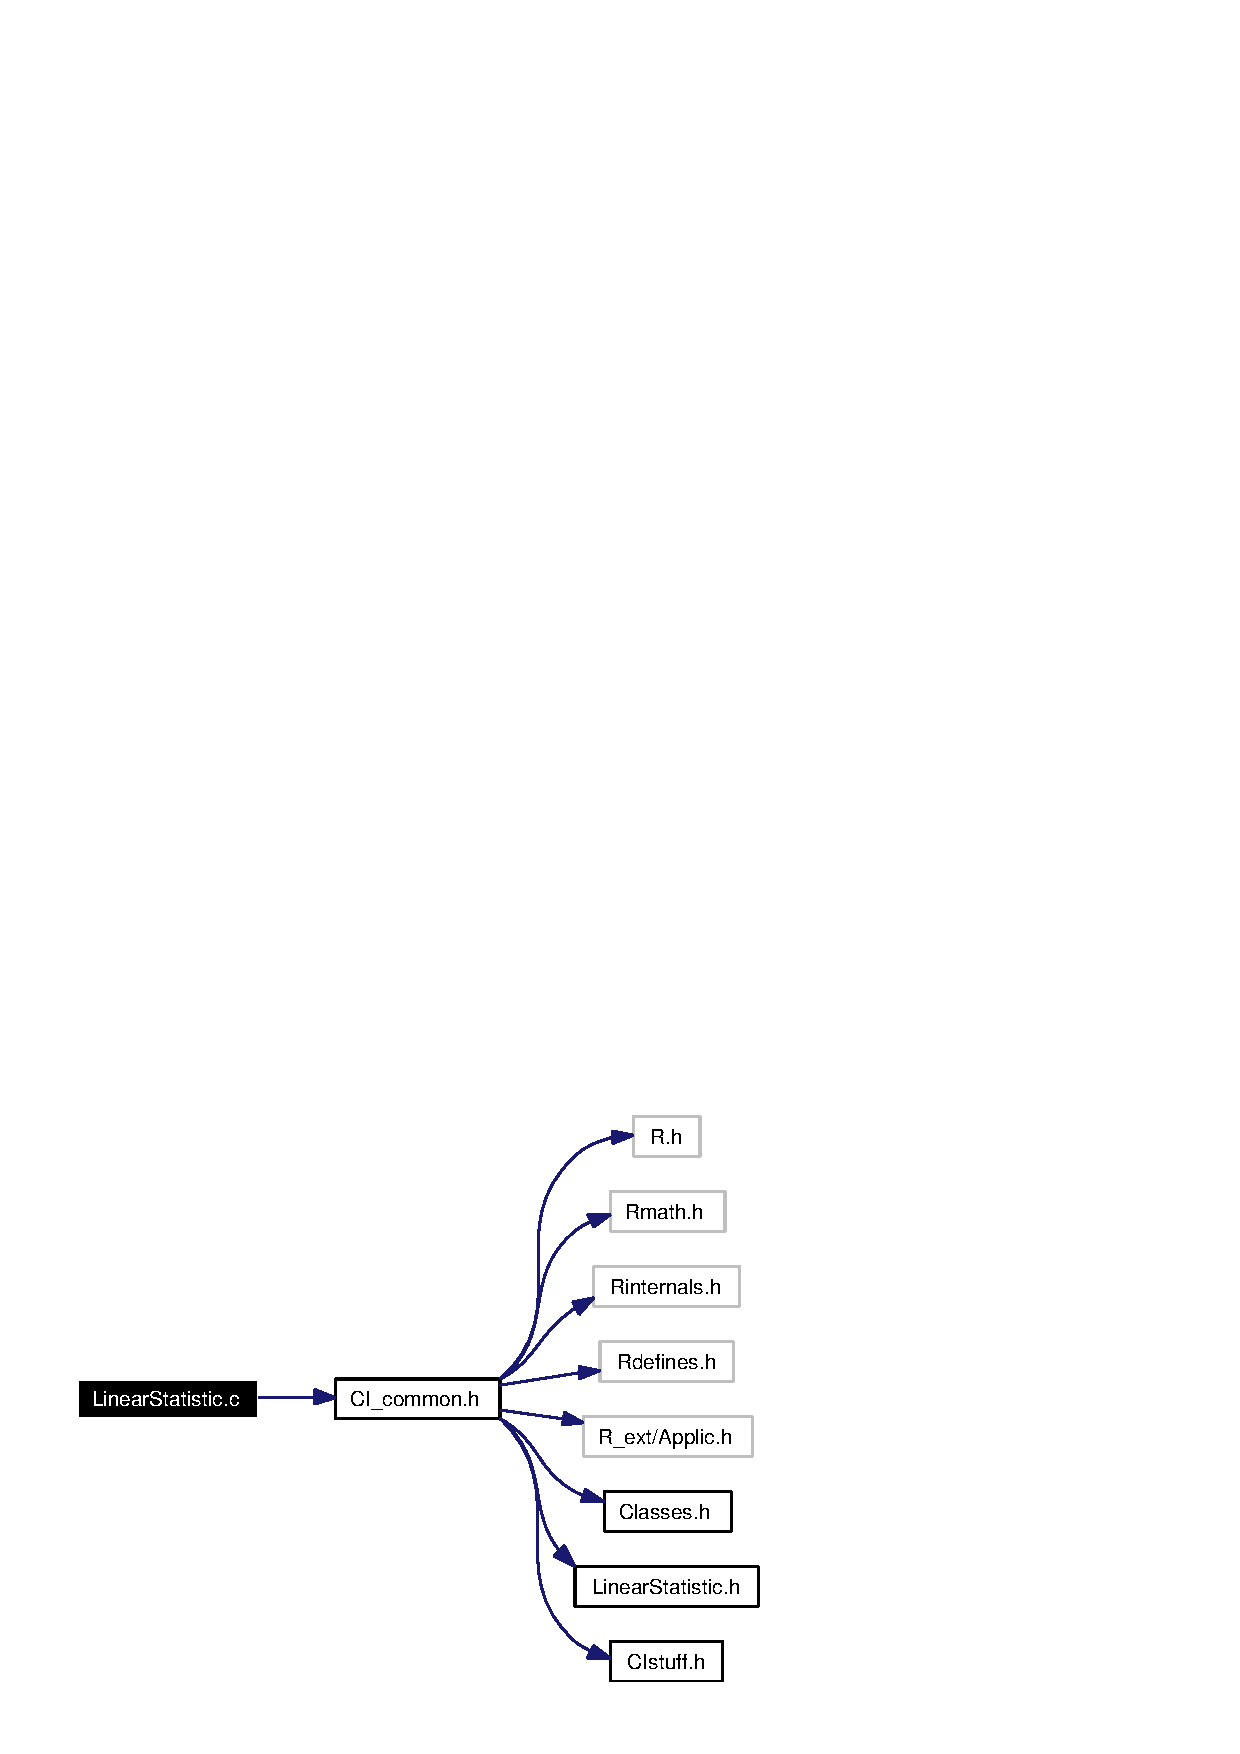
\includegraphics[width=400pt]{LinearStatistic_8c__incl}
\end{center}
\end{figure}
\subsection*{Functions}
\begin{DoxyCompactItemize}
\item 
void \hyperlink{LinearStatistic_8c_a12e882779ecd0445c3a0dd9ac85dfeee}{C\_\-kronecker} (const double $\ast$A, const int m, const int n, const double $\ast$B, const int r, const int s, double $\ast$ans)
\item 
SEXP \hyperlink{LinearStatistic_8c_a95f5ed4c75d42e2e98ed09c9c9d48ff5}{R\_\-kronecker} (SEXP A, SEXP B)
\item 
void \hyperlink{LinearStatistic_8c_ae2f62abe13ee5b625141b5d4a496d832}{C\_\-ExpectCovarInfluence} (const double $\ast$y, const int q, const double $\ast$weights, const int n, SEXP ans)
\item 
SEXP \hyperlink{LinearStatistic_8c_a6216ea560644c08002fb32756ae67dcc}{R\_\-ExpectCovarInfluence} (SEXP y, SEXP weights)
\item 
void \hyperlink{LinearStatistic_8c_a94a0805ea258af79d426c095feee399a}{C\_\-ExpectCovarLinearStatistic} (const double $\ast$x, const int p, const double $\ast$y, const int q, const double $\ast$weights, const int n, const SEXP expcovinf, SEXP ans)
\item 
SEXP \hyperlink{LinearStatistic_8c_a58fff8082d3ab197994a21a10c422353}{R\_\-ExpectCovarLinearStatistic} (SEXP x, SEXP y, SEXP weights, SEXP expcovinf)
\item 
void \hyperlink{LinearStatistic_8c_aaefa2a9406bb30b323715e3db41da637}{C\_\-LinearStatistic} (const double $\ast$x, const int p, const double $\ast$y, const int q, const double $\ast$weights, const int n, double $\ast$ans)
\item 
SEXP \hyperlink{LinearStatistic_8c_a732bfc8e1797d8953482aa31f9b43e5f}{R\_\-LinearStatistic} (SEXP x, SEXP y, SEXP weights)
\item 
void \hyperlink{LinearStatistic_8c_aa34b0f12fac36231a105d6dc903bfe89}{C\_\-PermutedLinearStatistic} (const double $\ast$x, const int p, const double $\ast$y, const int q, const int n, const int nperm, const int $\ast$indx, const int $\ast$perm, double $\ast$ans)
\item 
SEXP \hyperlink{LinearStatistic_8c_abe383bcae17e8b3a1d5740ec16a9817a}{R\_\-PermutedLinearStatistic} (SEXP x, SEXP y, SEXP indx, SEXP perm)
\end{DoxyCompactItemize}


\subsection{Detailed Description}
Linear statistics for conditional inference

\begin{DoxyAuthor}{Author}

\end{DoxyAuthor}
\begin{DoxyParagraph}{Author:}
hothorn 
\end{DoxyParagraph}
\begin{DoxyDate}{Date}

\end{DoxyDate}
\begin{DoxyParagraph}{Date:}
2007-\/02-\/15 09:25:46 +0100 (Thu, 15 Feb 2007) 
\end{DoxyParagraph}


Definition in file \hyperlink{LinearStatistic_8c_source}{LinearStatistic.c}.



\subsection{Function Documentation}
\hypertarget{LinearStatistic_8c_ae2f62abe13ee5b625141b5d4a496d832}{
\index{LinearStatistic.c@{LinearStatistic.c}!C\_\-ExpectCovarInfluence@{C\_\-ExpectCovarInfluence}}
\index{C\_\-ExpectCovarInfluence@{C\_\-ExpectCovarInfluence}!LinearStatistic.c@{LinearStatistic.c}}
\subsubsection[{C\_\-ExpectCovarInfluence}]{\setlength{\rightskip}{0pt plus 5cm}void C\_\-ExpectCovarInfluence (
\begin{DoxyParamCaption}
\item[{const double $\ast$}]{ y, }
\item[{const int}]{ q, }
\item[{const double $\ast$}]{ weights, }
\item[{const int}]{ n, }
\item[{SEXP}]{ ans}
\end{DoxyParamCaption}
)}}
\label{LinearStatistic_8c_ae2f62abe13ee5b625141b5d4a496d832}
Conditional expectation and covariance of the influence function\par
 
\begin{DoxyParams}{Parameters}
\item[{\em y}]values of the influence function \item[{\em q}]dimension of the influence function \item[{\em weights}]case weights \item[{\em n}]number of observations \item[{\em ans}]return value; an object of class `ExpectCovarInfluence' \end{DoxyParams}


Definition at line 80 of file LinearStatistic.c.



References coin\_\-covarianceSym, coin\_\-expectationSym, and coin\_\-sumweightsSym.



Referenced by R\_\-ExpectCovarInfluence().

\hypertarget{LinearStatistic_8c_a94a0805ea258af79d426c095feee399a}{
\index{LinearStatistic.c@{LinearStatistic.c}!C\_\-ExpectCovarLinearStatistic@{C\_\-ExpectCovarLinearStatistic}}
\index{C\_\-ExpectCovarLinearStatistic@{C\_\-ExpectCovarLinearStatistic}!LinearStatistic.c@{LinearStatistic.c}}
\subsubsection[{C\_\-ExpectCovarLinearStatistic}]{\setlength{\rightskip}{0pt plus 5cm}void C\_\-ExpectCovarLinearStatistic (
\begin{DoxyParamCaption}
\item[{const double $\ast$}]{ x, }
\item[{const int}]{ p, }
\item[{const double $\ast$}]{ y, }
\item[{const int}]{ q, }
\item[{const double $\ast$}]{ weights, }
\item[{const int}]{ n, }
\item[{const SEXP}]{ expcovinf, }
\item[{SEXP}]{ ans}
\end{DoxyParamCaption}
)}}
\label{LinearStatistic_8c_a94a0805ea258af79d426c095feee399a}
Conditional expectation and covariance of the a linear statistic\par
 
\begin{DoxyParams}{Parameters}
\item[{\em x}]values of the transformation \item[{\em p}]dimension of the transformation \item[{\em y}]values of the influence function \item[{\em q}]dimension of the influence function \item[{\em weights}]case weights \item[{\em n}]number of observations \item[{\em expcovinf}]an object of class `ExpectCovarInfluence' \item[{\em ans}]return value; an object of class `ExpectCovar' \end{DoxyParams}


Definition at line 192 of file LinearStatistic.c.



References C\_\-kronecker(), coin\_\-covarianceSym, coin\_\-expectationSym, and coin\_\-sumweightsSym.



Referenced by R\_\-ExpectCovarLinearStatistic().



Here is the call graph for this function:
\nopagebreak
\begin{figure}[H]
\begin{center}
\leavevmode
\includegraphics[width=350pt]{LinearStatistic_8c_a94a0805ea258af79d426c095feee399a_cgraph}
\end{center}
\end{figure}


\hypertarget{LinearStatistic_8c_a12e882779ecd0445c3a0dd9ac85dfeee}{
\index{LinearStatistic.c@{LinearStatistic.c}!C\_\-kronecker@{C\_\-kronecker}}
\index{C\_\-kronecker@{C\_\-kronecker}!LinearStatistic.c@{LinearStatistic.c}}
\subsubsection[{C\_\-kronecker}]{\setlength{\rightskip}{0pt plus 5cm}void C\_\-kronecker (
\begin{DoxyParamCaption}
\item[{const double $\ast$}]{ A, }
\item[{const int}]{ m, }
\item[{const int}]{ n, }
\item[{const double $\ast$}]{ B, }
\item[{const int}]{ r, }
\item[{const int}]{ s, }
\item[{double $\ast$}]{ ans}
\end{DoxyParamCaption}
)}}
\label{LinearStatistic_8c_a12e882779ecd0445c3a0dd9ac85dfeee}
Computes the Kronecker product of two matrices\par
 
\begin{DoxyParams}{Parameters}
\item[{\em A}]matrix \item[{\em m}]nrow(A) \item[{\em n}]ncol(A) \item[{\em B}]matrix \item[{\em r}]nrow(B) \item[{\em s}]ncol(B) \item[{\em ans}]return value; a pointer to a REALSXP-\/vector of length (mr x ns) \end{DoxyParams}


Definition at line 22 of file LinearStatistic.c.



Referenced by C\_\-ExpectCovarLinearStatistic(), and R\_\-kronecker().

\hypertarget{LinearStatistic_8c_aaefa2a9406bb30b323715e3db41da637}{
\index{LinearStatistic.c@{LinearStatistic.c}!C\_\-LinearStatistic@{C\_\-LinearStatistic}}
\index{C\_\-LinearStatistic@{C\_\-LinearStatistic}!LinearStatistic.c@{LinearStatistic.c}}
\subsubsection[{C\_\-LinearStatistic}]{\setlength{\rightskip}{0pt plus 5cm}void C\_\-LinearStatistic (
\begin{DoxyParamCaption}
\item[{const double $\ast$}]{ x, }
\item[{const int}]{ p, }
\item[{const double $\ast$}]{ y, }
\item[{const int}]{ q, }
\item[{const double $\ast$}]{ weights, }
\item[{const int}]{ n, }
\item[{double $\ast$}]{ ans}
\end{DoxyParamCaption}
)}}
\label{LinearStatistic_8c_aaefa2a9406bb30b323715e3db41da637}
Computes the linear statistic, formula (1) in the paper\par
 
\begin{DoxyParams}{Parameters}
\item[{\em x}]values of the transformation \item[{\em p}]dimension of the transformation \item[{\em y}]values of the influence function \item[{\em q}]dimension of the influence function \item[{\em weights}]case weights \item[{\em n}]number of observations \item[{\em ans}]return value; a pointer to a REALSXP-\/vector of length pq \end{DoxyParams}


Definition at line 327 of file LinearStatistic.c.



Referenced by R\_\-LinearStatistic().

\hypertarget{LinearStatistic_8c_aa34b0f12fac36231a105d6dc903bfe89}{
\index{LinearStatistic.c@{LinearStatistic.c}!C\_\-PermutedLinearStatistic@{C\_\-PermutedLinearStatistic}}
\index{C\_\-PermutedLinearStatistic@{C\_\-PermutedLinearStatistic}!LinearStatistic.c@{LinearStatistic.c}}
\subsubsection[{C\_\-PermutedLinearStatistic}]{\setlength{\rightskip}{0pt plus 5cm}void C\_\-PermutedLinearStatistic (
\begin{DoxyParamCaption}
\item[{const double $\ast$}]{ x, }
\item[{const int}]{ p, }
\item[{const double $\ast$}]{ y, }
\item[{const int}]{ q, }
\item[{const int}]{ n, }
\item[{const int}]{ nperm, }
\item[{const int $\ast$}]{ indx, }
\item[{const int $\ast$}]{ perm, }
\item[{double $\ast$}]{ ans}
\end{DoxyParamCaption}
)}}
\label{LinearStatistic_8c_aa34b0f12fac36231a105d6dc903bfe89}
Linear Statistic with permuted indices\par
 
\begin{DoxyParams}{Parameters}
\item[{\em x}]values of the transformation \item[{\em p}]dimension of the transformation \item[{\em y}]values of the influence function \item[{\em q}]dimension of the influence function \item[{\em n}]number of observations \item[{\em nperm}]number of permutations \item[{\em indx}]indices for the x-\/part \item[{\em perm}](permuted) indices for the y-\/part \item[{\em ans}]return value; a pointer to a REALSXP-\/vector of length pq \end{DoxyParams}


Definition at line 409 of file LinearStatistic.c.



Referenced by R\_\-MonteCarloIndependenceTest(), and R\_\-PermutedLinearStatistic().

\hypertarget{LinearStatistic_8c_a6216ea560644c08002fb32756ae67dcc}{
\index{LinearStatistic.c@{LinearStatistic.c}!R\_\-ExpectCovarInfluence@{R\_\-ExpectCovarInfluence}}
\index{R\_\-ExpectCovarInfluence@{R\_\-ExpectCovarInfluence}!LinearStatistic.c@{LinearStatistic.c}}
\subsubsection[{R\_\-ExpectCovarInfluence}]{\setlength{\rightskip}{0pt plus 5cm}SEXP R\_\-ExpectCovarInfluence (
\begin{DoxyParamCaption}
\item[{SEXP}]{ y, }
\item[{SEXP}]{ weights}
\end{DoxyParamCaption}
)}}
\label{LinearStatistic_8c_a6216ea560644c08002fb32756ae67dcc}
R-\/interface to C\_\-ExpectCovarInfluence\par
 
\begin{DoxyParams}{Parameters}
\item[{\em y}]values of the influence function \item[{\em weights}]case weights \end{DoxyParams}


Definition at line 150 of file LinearStatistic.c.



References C\_\-ExpectCovarInfluence(), coin\_\-covarianceSym, coin\_\-expectationSym, coin\_\-sumweightsSym, ncol(), and nrow().



Here is the call graph for this function:
\nopagebreak
\begin{figure}[H]
\begin{center}
\leavevmode
\includegraphics[width=380pt]{LinearStatistic_8c_a6216ea560644c08002fb32756ae67dcc_cgraph}
\end{center}
\end{figure}


\hypertarget{LinearStatistic_8c_a58fff8082d3ab197994a21a10c422353}{
\index{LinearStatistic.c@{LinearStatistic.c}!R\_\-ExpectCovarLinearStatistic@{R\_\-ExpectCovarLinearStatistic}}
\index{R\_\-ExpectCovarLinearStatistic@{R\_\-ExpectCovarLinearStatistic}!LinearStatistic.c@{LinearStatistic.c}}
\subsubsection[{R\_\-ExpectCovarLinearStatistic}]{\setlength{\rightskip}{0pt plus 5cm}SEXP R\_\-ExpectCovarLinearStatistic (
\begin{DoxyParamCaption}
\item[{SEXP}]{ x, }
\item[{SEXP}]{ y, }
\item[{SEXP}]{ weights, }
\item[{SEXP}]{ expcovinf}
\end{DoxyParamCaption}
)}}
\label{LinearStatistic_8c_a58fff8082d3ab197994a21a10c422353}
R-\/interface to C\_\-ExpectCovarLinearStatistic\par
 
\begin{DoxyParams}{Parameters}
\item[{\em x}]values of the transformation \item[{\em y}]values of the influence function \item[{\em weights}]case weights \item[{\em expcovinf}]an object of class `ExpectCovarInfluence' \end{DoxyParams}


Definition at line 285 of file LinearStatistic.c.



References C\_\-ExpectCovarLinearStatistic(), coin\_\-covarianceSym, coin\_\-expectationSym, ncol(), and nrow().



Here is the call graph for this function:
\nopagebreak
\begin{figure}[H]
\begin{center}
\leavevmode
\includegraphics[width=400pt]{LinearStatistic_8c_a58fff8082d3ab197994a21a10c422353_cgraph}
\end{center}
\end{figure}


\hypertarget{LinearStatistic_8c_a95f5ed4c75d42e2e98ed09c9c9d48ff5}{
\index{LinearStatistic.c@{LinearStatistic.c}!R\_\-kronecker@{R\_\-kronecker}}
\index{R\_\-kronecker@{R\_\-kronecker}!LinearStatistic.c@{LinearStatistic.c}}
\subsubsection[{R\_\-kronecker}]{\setlength{\rightskip}{0pt plus 5cm}SEXP R\_\-kronecker (
\begin{DoxyParamCaption}
\item[{SEXP}]{ A, }
\item[{SEXP}]{ B}
\end{DoxyParamCaption}
)}}
\label{LinearStatistic_8c_a95f5ed4c75d42e2e98ed09c9c9d48ff5}
R-\/interface to C\_\-kronecker\par
 
\begin{DoxyParams}{Parameters}
\item[{\em A}]matrix \item[{\em B}]matrix \end{DoxyParams}


Definition at line 51 of file LinearStatistic.c.



References C\_\-kronecker(), ncol(), and nrow().



Here is the call graph for this function:
\nopagebreak
\begin{figure}[H]
\begin{center}
\leavevmode
\includegraphics[width=268pt]{LinearStatistic_8c_a95f5ed4c75d42e2e98ed09c9c9d48ff5_cgraph}
\end{center}
\end{figure}


\hypertarget{LinearStatistic_8c_a732bfc8e1797d8953482aa31f9b43e5f}{
\index{LinearStatistic.c@{LinearStatistic.c}!R\_\-LinearStatistic@{R\_\-LinearStatistic}}
\index{R\_\-LinearStatistic@{R\_\-LinearStatistic}!LinearStatistic.c@{LinearStatistic.c}}
\subsubsection[{R\_\-LinearStatistic}]{\setlength{\rightskip}{0pt plus 5cm}SEXP R\_\-LinearStatistic (
\begin{DoxyParamCaption}
\item[{SEXP}]{ x, }
\item[{SEXP}]{ y, }
\item[{SEXP}]{ weights}
\end{DoxyParamCaption}
)}}
\label{LinearStatistic_8c_a732bfc8e1797d8953482aa31f9b43e5f}
R-\/interface to C\_\-LinearStatistic \par
 
\begin{DoxyParams}{Parameters}
\item[{\em x}]values of the transformation \item[{\em y}]values of the influence function \item[{\em weights}]case weights \end{DoxyParams}


Definition at line 363 of file LinearStatistic.c.



References C\_\-LinearStatistic(), ncol(), and nrow().



Here is the call graph for this function:
\nopagebreak
\begin{figure}[H]
\begin{center}
\leavevmode
\includegraphics[width=310pt]{LinearStatistic_8c_a732bfc8e1797d8953482aa31f9b43e5f_cgraph}
\end{center}
\end{figure}


\hypertarget{LinearStatistic_8c_abe383bcae17e8b3a1d5740ec16a9817a}{
\index{LinearStatistic.c@{LinearStatistic.c}!R\_\-PermutedLinearStatistic@{R\_\-PermutedLinearStatistic}}
\index{R\_\-PermutedLinearStatistic@{R\_\-PermutedLinearStatistic}!LinearStatistic.c@{LinearStatistic.c}}
\subsubsection[{R\_\-PermutedLinearStatistic}]{\setlength{\rightskip}{0pt plus 5cm}SEXP R\_\-PermutedLinearStatistic (
\begin{DoxyParamCaption}
\item[{SEXP}]{ x, }
\item[{SEXP}]{ y, }
\item[{SEXP}]{ indx, }
\item[{SEXP}]{ perm}
\end{DoxyParamCaption}
)}}
\label{LinearStatistic_8c_abe383bcae17e8b3a1d5740ec16a9817a}
Linear Statistic with permuted indices\par
 
\begin{DoxyParams}{Parameters}
\item[{\em x}]values of the transformation \item[{\em y}]values of the influence function \item[{\em indx}]indices for the x-\/part \item[{\em perm}](permuted) indices for the y-\/part \end{DoxyParams}


Definition at line 442 of file LinearStatistic.c.



References C\_\-PermutedLinearStatistic(), ncol(), and nrow().



Here is the call graph for this function:
\nopagebreak
\begin{figure}[H]
\begin{center}
\leavevmode
\includegraphics[width=400pt]{LinearStatistic_8c_abe383bcae17e8b3a1d5740ec16a9817a_cgraph}
\end{center}
\end{figure}



\hypertarget{LinearStatistic_8d}{
\section{Linear\-Statistic.d File Reference}
\label{LinearStatistic_8d}\index{LinearStatistic.d@{LinearStatistic.d}}
}

\hypertarget{LinearStatistic_8h}{
\section{Linear\-Statistic.h File Reference}
\label{LinearStatistic_8h}\index{LinearStatistic.h@{LinearStatistic.h}}
}


This graph shows which files directly or indirectly include this file:\begin{figure}[H]
\begin{center}
\leavevmode
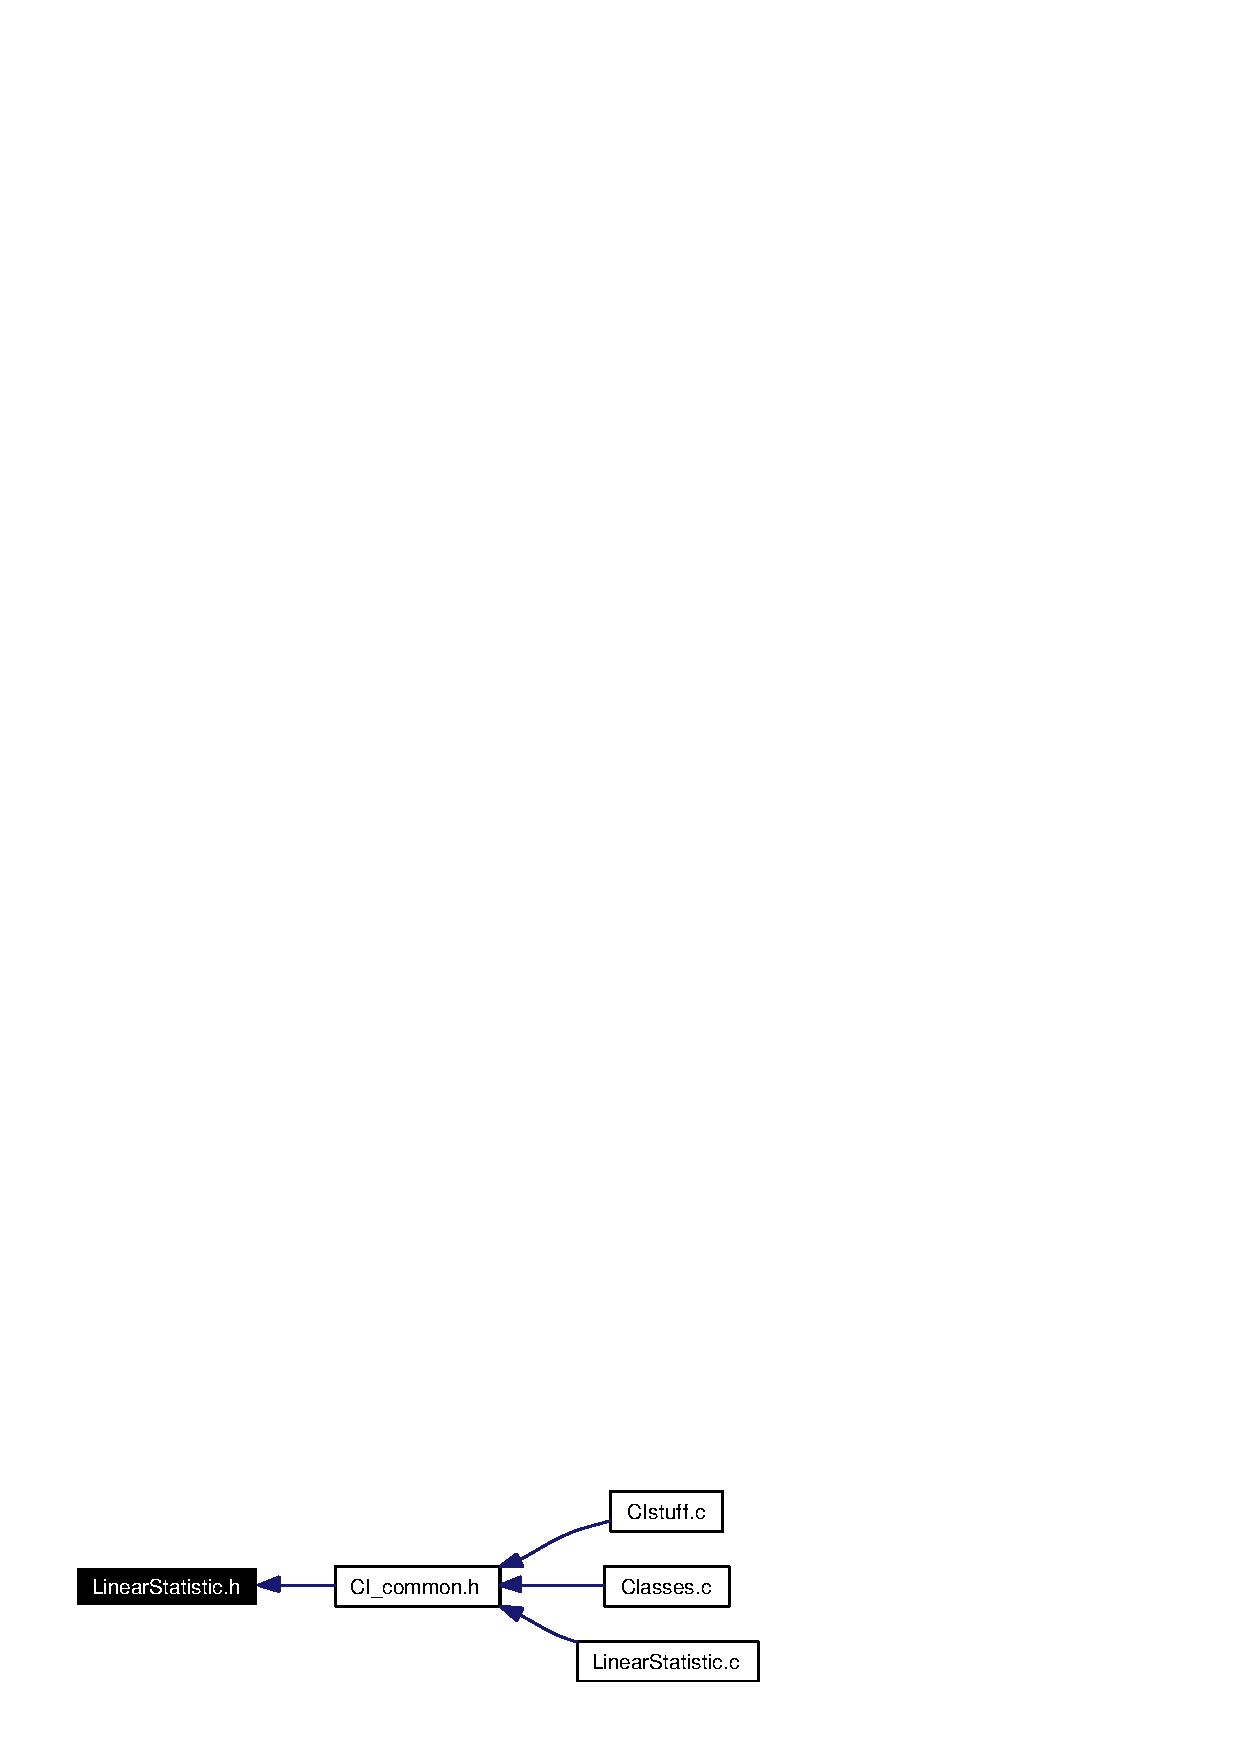
\includegraphics[width=182pt]{LinearStatistic_8h__dep__incl}
\end{center}
\end{figure}
\subsection*{Functions}
\begin{CompactItemize}
\item 
void \hyperlink{LinearStatistic_8h_a34b0f12fac36231a105d6dc903bfe89}{C\_\-Permuted\-Linear\-Statistic} (const double $\ast$x, const int p, const double $\ast$y, const int q, const int n, const int nperm, const int $\ast$indx, const int $\ast$perm, double $\ast$ans)
\end{CompactItemize}


\subsection{Function Documentation}
\hypertarget{LinearStatistic_8h_a34b0f12fac36231a105d6dc903bfe89}{
\index{LinearStatistic.h@{Linear\-Statistic.h}!C_PermutedLinearStatistic@{C\_\-PermutedLinearStatistic}}
\index{C_PermutedLinearStatistic@{C\_\-PermutedLinearStatistic}!LinearStatistic.h@{Linear\-Statistic.h}}
\subsubsection[C\_\-PermutedLinearStatistic]{\setlength{\rightskip}{0pt plus 5cm}void C\_\-Permuted\-Linear\-Statistic (const double $\ast$ {\em x}, const int {\em p}, const double $\ast$ {\em y}, const int {\em q}, const int {\em n}, const int {\em nperm}, const int $\ast$ {\em indx}, const int $\ast$ {\em perm}, double $\ast$ {\em ans})}}
\label{LinearStatistic_8h_a34b0f12fac36231a105d6dc903bfe89}


Linear Statistic with permuted indices\par
 \begin{Desc}
\item[Parameters:]
\begin{description}
\item[{\em x}]values of the transformation \item[{\em p}]dimension of the transformation \item[{\em y}]values of the influence function \item[{\em q}]dimension of the influence function \item[{\em n}]number of observations \item[{\em nperm}]number of permutations \item[{\em indx}]indices for the x-part \item[{\em perm}](permuted) indices for the y-part \item[{\em ans}]return value; a pointer to a REALSXP-vector of length pq \end{description}
\end{Desc}


Definition at line 409 of file Linear\-Statistic.c.

Referenced by R\_\-Monte\-Carlo\-Independence\-Test().
\hypertarget{StreitbergRoehmel_8c}{
\section{Streitberg\-Roehmel.c File Reference}
\label{StreitbergRoehmel_8c}\index{StreitbergRoehmel.c@{StreitbergRoehmel.c}}
}
{\tt \#include $<$R.h$>$}\par
{\tt \#include $<$Rmath.h$>$}\par
{\tt \#include $<$Rdefines.h$>$}\par


Include dependency graph for Streitberg\-Roehmel.c:\begin{figure}[H]
\begin{center}
\leavevmode
\includegraphics[width=127pt]{StreitbergRoehmel_8c__incl}
\end{center}
\end{figure}
\subsection*{Defines}
\begin{CompactItemize}
\item 
\#define \hyperlink{StreitbergRoehmel_8c_a0}{PERM\_\-MAX\_\-N}~1000000
\end{CompactItemize}
\subsection*{Functions}
\begin{CompactItemize}
\item 
SEXP \hyperlink{StreitbergRoehmel_8c_a1}{R\_\-cpermdist2} (SEXP score\_\-a, SEXP score\_\-b, SEXP m\_\-a, SEXP m\_\-b, SEXP ret\-Prob)
\end{CompactItemize}


\subsection{Detailed Description}
Exact Distribution of Two-Sample Permutation Tests Streitberg \& Roehmel Algorithm

\begin{Desc}
\item[Author:]\begin{Desc}
\item[Author]hothorn \end{Desc}
\end{Desc}
\begin{Desc}
\item[Date:]\begin{Desc}
\item[Date]2005/07/28 15:04:29 \end{Desc}
\end{Desc}


Definition in file \hyperlink{StreitbergRoehmel_8c-source}{Streitberg\-Roehmel.c}.

\subsection{Define Documentation}
\hypertarget{StreitbergRoehmel_8c_a0}{
\index{StreitbergRoehmel.c@{Streitberg\-Roehmel.c}!PERM_MAX_N@{PERM\_\-MAX\_\-N}}
\index{PERM_MAX_N@{PERM\_\-MAX\_\-N}!StreitbergRoehmel.c@{Streitberg\-Roehmel.c}}
\subsubsection[PERM\_\-MAX\_\-N]{\setlength{\rightskip}{0pt plus 5cm}\#define PERM\_\-MAX\_\-N~1000000}}
\label{StreitbergRoehmel_8c_a0}




Definition at line 19 of file Streitberg\-Roehmel.c.

Referenced by R\_\-cpermdist2().

\subsection{Function Documentation}
\hypertarget{StreitbergRoehmel_8c_a1}{
\index{StreitbergRoehmel.c@{Streitberg\-Roehmel.c}!R_cpermdist2@{R\_\-cpermdist2}}
\index{R_cpermdist2@{R\_\-cpermdist2}!StreitbergRoehmel.c@{Streitberg\-Roehmel.c}}
\subsubsection[R\_\-cpermdist2]{\setlength{\rightskip}{0pt plus 5cm}SEXP R\_\-cpermdist2 (SEXP {\em score\_\-a}, SEXP {\em score\_\-b}, SEXP {\em m\_\-a}, SEXP {\em m\_\-b}, SEXP {\em ret\-Prob})}}
\label{StreitbergRoehmel_8c_a1}


The density of the permutation distribution for the independent two sample problem.

REFERENCES

Bernd Streitberg \& Joachim R$\backslash$\char`\"{}ohmel (1986), Exact distributions for permutations and rank tests: An introduction to some recently published algorithms. Statistical Software Newsletter 12(1), 10-17.

Bernd Streitberg \& Joachim R$\backslash$\char`\"{}ohmel (1987), Exakte Verteilungen f$\backslash$\char`\"{}ur Rang- und Randomisierungstests im allgemeinen \$c\$-Stichprobenfall. EDV in Medizin und Biologie 18(1), 12-19 (in german).

\begin{Desc}
\item[Parameters:]
\begin{description}
\item[{\em score\_\-a}]score vector (typically c(1,1,...,1)) \item[{\em score\_\-b}]score vector (typically ranks) \item[{\em m\_\-a}]integer indicating the sum of m\_\-a elements of score\_\-a \item[{\em m\_\-b}]integer indicating the sum of m\_\-b elements of score\_\-b \item[{\em ret\-Prob}]logical indicating whether the density (TRUE) or the matrix of all permutations should be returned \end{description}
\end{Desc}


Definition at line 46 of file Streitberg\-Roehmel.c.

References PERM\_\-MAX\_\-N.
\hypertarget{StreitbergRoehmel_8d}{
\section{Streitberg\-Roehmel.d File Reference}
\label{StreitbergRoehmel_8d}\index{StreitbergRoehmel.d@{StreitbergRoehmel.d}}
}

\hypertarget{vandeWiel_8c}{
\section{vande\-Wiel.c File Reference}
\label{vandeWiel_8c}\index{vandeWiel.c@{vandeWiel.c}}
}
{\tt \#include $<$R.h$>$}\par
{\tt \#include $<$Rmath.h$>$}\par
{\tt \#include $<$Rdefines.h$>$}\par


Include dependency graph for vande\-Wiel.c:\begin{figure}[H]
\begin{center}
\leavevmode
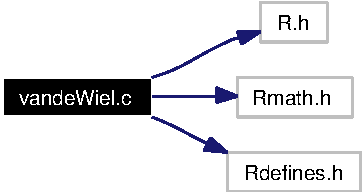
\includegraphics[width=104pt]{vandeWiel_8c__incl}
\end{center}
\end{figure}
\subsection*{Functions}
\begin{CompactItemize}
\item 
double \hyperlink{vandeWiel_8c_a0}{binomi} (int m, int n)
\item 
\hyperlink{structcelW}{cel\-W} $\ast$$\ast$ \hyperlink{vandeWiel_8c_a1}{reserve\-W} (int a, int b)
\item 
void \hyperlink{vandeWiel_8c_a2}{Free\-W} (int a, \hyperlink{structcelW}{cel\-W} $\ast$$\ast$W)
\item 
void \hyperlink{vandeWiel_8c_a3}{init\-W} (int a, int b, \hyperlink{structcelW}{cel\-W} $\ast$$\ast$W)
\item 
void \hyperlink{vandeWiel_8c_a4}{mult} (\hyperlink{structcelW}{cel\-W} $\ast$tem, int a, int b, int rank, double $\ast$rs)
\item 
void \hyperlink{vandeWiel_8c_a5}{plus} (\hyperlink{structcelW}{cel\-W} $\ast$$\ast$W, \hyperlink{structcelW}{cel\-W} $\ast$tempie, int a, int b)
\item 
void \hyperlink{vandeWiel_8c_a6}{mymergesort} (\hyperlink{structcelW}{cel\-W} temptw, long tijd)
\item 
void \hyperlink{vandeWiel_8c_a7}{fillcell} (\hyperlink{structcelW}{cel\-W} $\ast$$\ast$W, int i1, int j1, int r, double $\ast$rs)
\item 
void \hyperlink{vandeWiel_8c_a8}{mirror\-W} (\hyperlink{structcelW}{cel\-W} $\ast$$\ast$W, int ce, int bep, int start, double $\ast$rs)
\item 
void \hyperlink{vandeWiel_8c_a9}{make\-W} (\hyperlink{structcelW}{cel\-W} $\ast$$\ast$W, int a, int b, int start, double $\ast$rs)
\item 
void \hyperlink{vandeWiel_8c_a10}{cumulcoef} (\hyperlink{structcelW}{cel\-W} $\ast$$\ast$W, int i1, int j1)
\item 
double \hyperlink{vandeWiel_8c_a11}{numbersmall} (int c, int b, double ob, \hyperlink{structcelW}{cel\-W} $\ast$$\ast$W1, \hyperlink{structcelW}{cel\-W} $\ast$$\ast$W2)
\item 
SEXP \hyperlink{vandeWiel_8c_a12}{R\_\-split\_\-up\_\-2sample} (SEXP scores, SEXP m, SEXP obs)
\end{CompactItemize}


\subsection{Detailed Description}
Exact Distribution of Two-Sample Permutation Tests van de Wiel split-up Algorithm

Author: Mark van de Wiel (2001-2005) $<$\href{mailto:m.a.v.d.wiel@TUE.nl}{\tt m.a.v.d.wiel@TUE.nl}$>$ with modifications for R by Torsten Hothorn $<$\href{mailto:Torsten.Hothorn@R-project.org}{\tt Torsten.Hothorn@R-project.org}$>$

\begin{Desc}
\item[Author:]\begin{Desc}
\item[Author]hothorn \end{Desc}
\end{Desc}
\begin{Desc}
\item[Date:]\begin{Desc}
\item[Date]2005/07/28 15:04:29 \end{Desc}
\end{Desc}


Definition in file \hyperlink{vandeWiel_8c-source}{vande\-Wiel.c}.

\subsection{Function Documentation}
\hypertarget{vandeWiel_8c_a0}{
\index{vandeWiel.c@{vande\-Wiel.c}!binomi@{binomi}}
\index{binomi@{binomi}!vandeWiel.c@{vande\-Wiel.c}}
\subsubsection[binomi]{\setlength{\rightskip}{0pt plus 5cm}double binomi (int {\em m}, int {\em n})}}
\label{vandeWiel_8c_a0}




Definition at line 37 of file vande\-Wiel.c.

Referenced by R\_\-split\_\-up\_\-2sample(), and reserve\-W().\hypertarget{vandeWiel_8c_a10}{
\index{vandeWiel.c@{vande\-Wiel.c}!cumulcoef@{cumulcoef}}
\index{cumulcoef@{cumulcoef}!vandeWiel.c@{vande\-Wiel.c}}
\subsubsection[cumulcoef]{\setlength{\rightskip}{0pt plus 5cm}void cumulcoef (\hyperlink{structcelW}{cel\-W} $\ast$$\ast$ {\em W}, int {\em i1}, int {\em j1})}}
\label{vandeWiel_8c_a10}




Definition at line 316 of file vande\-Wiel.c.

References cel\-W::c, and cel\-W::length.

Referenced by R\_\-split\_\-up\_\-2sample().\hypertarget{vandeWiel_8c_a7}{
\index{vandeWiel.c@{vande\-Wiel.c}!fillcell@{fillcell}}
\index{fillcell@{fillcell}!vandeWiel.c@{vande\-Wiel.c}}
\subsubsection[fillcell]{\setlength{\rightskip}{0pt plus 5cm}void fillcell (\hyperlink{structcelW}{cel\-W} $\ast$$\ast$ {\em W}, int {\em i1}, int {\em j1}, int {\em r}, double $\ast$ {\em rs})}}
\label{vandeWiel_8c_a7}




Definition at line 211 of file vande\-Wiel.c.

References cel\-W::c, cel\-W::length, mult(), mymergesort(), plus(), and cel\-W::x.

Referenced by make\-W().

Here is the call graph for this function:\begin{figure}[H]
\begin{center}
\leavevmode
\includegraphics[width=95pt]{vandeWiel_8c_a7_cgraph}
\end{center}
\end{figure}
\hypertarget{vandeWiel_8c_a2}{
\index{vandeWiel.c@{vande\-Wiel.c}!FreeW@{FreeW}}
\index{FreeW@{FreeW}!vandeWiel.c@{vande\-Wiel.c}}
\subsubsection[FreeW]{\setlength{\rightskip}{0pt plus 5cm}void Free\-W (int {\em a}, \hyperlink{structcelW}{cel\-W} $\ast$$\ast$ {\em W})}}
\label{vandeWiel_8c_a2}




Definition at line 81 of file vande\-Wiel.c.

Referenced by R\_\-split\_\-up\_\-2sample().\hypertarget{vandeWiel_8c_a3}{
\index{vandeWiel.c@{vande\-Wiel.c}!initW@{initW}}
\index{initW@{initW}!vandeWiel.c@{vande\-Wiel.c}}
\subsubsection[initW]{\setlength{\rightskip}{0pt plus 5cm}void init\-W (int {\em a}, int {\em b}, \hyperlink{structcelW}{cel\-W} $\ast$$\ast$ {\em W})}}
\label{vandeWiel_8c_a3}




Definition at line 91 of file vande\-Wiel.c.

References cel\-W::c, cel\-W::length, and cel\-W::x.

Referenced by R\_\-split\_\-up\_\-2sample().\hypertarget{vandeWiel_8c_a9}{
\index{vandeWiel.c@{vande\-Wiel.c}!makeW@{makeW}}
\index{makeW@{makeW}!vandeWiel.c@{vande\-Wiel.c}}
\subsubsection[makeW]{\setlength{\rightskip}{0pt plus 5cm}void make\-W (\hyperlink{structcelW}{cel\-W} $\ast$$\ast$ {\em W}, int {\em a}, int {\em b}, int {\em start}, double $\ast$ {\em rs})}}
\label{vandeWiel_8c_a9}




Definition at line 281 of file vande\-Wiel.c.

References fillcell(), and mirror\-W().

Referenced by R\_\-split\_\-up\_\-2sample().

Here is the call graph for this function:\begin{figure}[H]
\begin{center}
\leavevmode
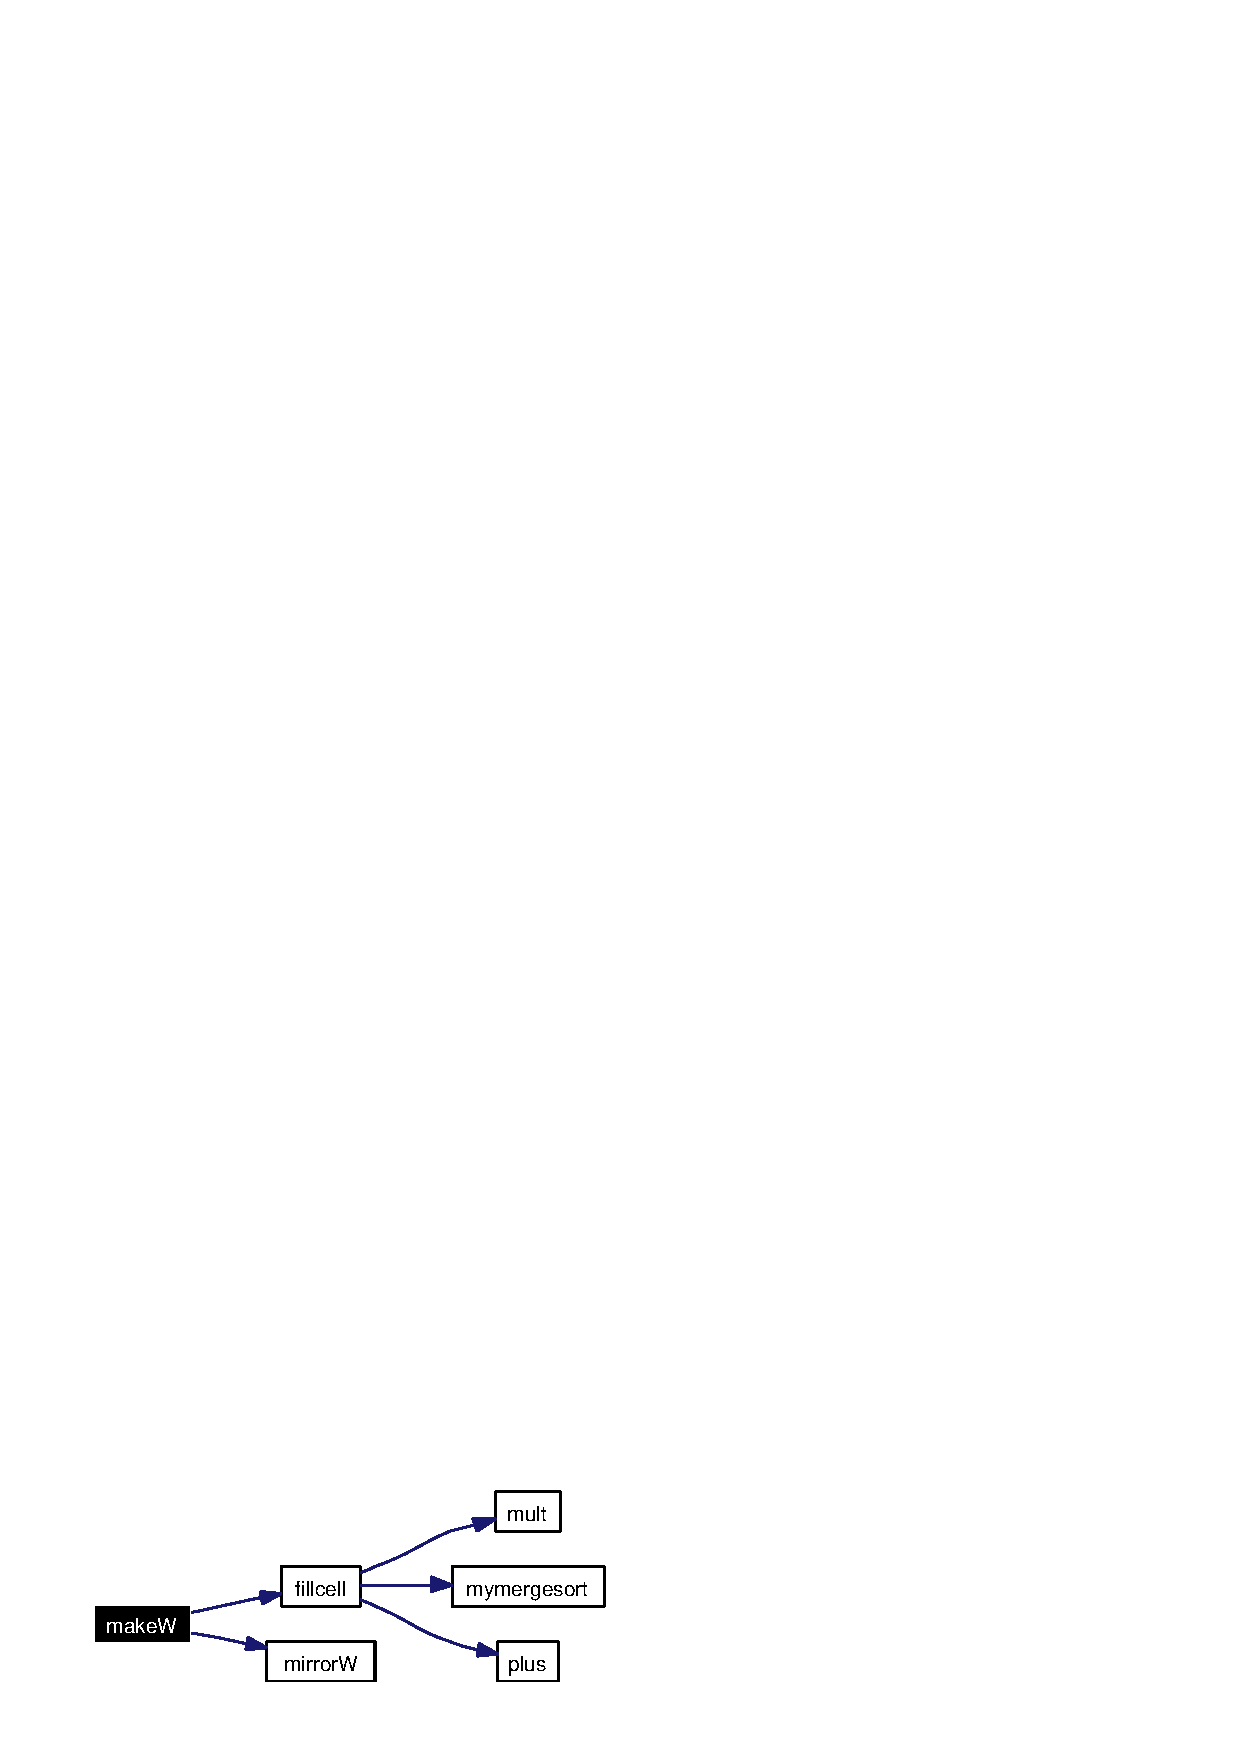
\includegraphics[width=144pt]{vandeWiel_8c_a9_cgraph}
\end{center}
\end{figure}
\hypertarget{vandeWiel_8c_a8}{
\index{vandeWiel.c@{vande\-Wiel.c}!mirrorW@{mirrorW}}
\index{mirrorW@{mirrorW}!vandeWiel.c@{vande\-Wiel.c}}
\subsubsection[mirrorW]{\setlength{\rightskip}{0pt plus 5cm}void mirror\-W (\hyperlink{structcelW}{cel\-W} $\ast$$\ast$ {\em W}, int {\em ce}, int {\em bep}, int {\em start}, double $\ast$ {\em rs})}}
\label{vandeWiel_8c_a8}




Definition at line 257 of file vande\-Wiel.c.

References cel\-W::c, cel\-W::length, and cel\-W::x.

Referenced by make\-W().\hypertarget{vandeWiel_8c_a4}{
\index{vandeWiel.c@{vande\-Wiel.c}!mult@{mult}}
\index{mult@{mult}!vandeWiel.c@{vande\-Wiel.c}}
\subsubsection[mult]{\setlength{\rightskip}{0pt plus 5cm}void mult (\hyperlink{structcelW}{cel\-W} $\ast$ {\em tem}, int {\em a}, int {\em b}, int {\em rank}, double $\ast$ {\em rs})}}
\label{vandeWiel_8c_a4}




Definition at line 106 of file vande\-Wiel.c.

References cel\-W::x.

Referenced by fillcell().\hypertarget{vandeWiel_8c_a6}{
\index{vandeWiel.c@{vande\-Wiel.c}!mymergesort@{mymergesort}}
\index{mymergesort@{mymergesort}!vandeWiel.c@{vande\-Wiel.c}}
\subsubsection[mymergesort]{\setlength{\rightskip}{0pt plus 5cm}void mymergesort (\hyperlink{structcelW}{cel\-W} {\em temptw}, long {\em tijd})}}
\label{vandeWiel_8c_a6}




Definition at line 159 of file vande\-Wiel.c.

References cel\-W::c, cel\-W::length, and cel\-W::x.

Referenced by fillcell().\hypertarget{vandeWiel_8c_a11}{
\index{vandeWiel.c@{vande\-Wiel.c}!numbersmall@{numbersmall}}
\index{numbersmall@{numbersmall}!vandeWiel.c@{vande\-Wiel.c}}
\subsubsection[numbersmall]{\setlength{\rightskip}{0pt plus 5cm}double numbersmall (int {\em c}, int {\em b}, double {\em ob}, \hyperlink{structcelW}{cel\-W} $\ast$$\ast$ {\em W1}, \hyperlink{structcelW}{cel\-W} $\ast$$\ast$ {\em W2})}}
\label{vandeWiel_8c_a11}




Definition at line 335 of file vande\-Wiel.c.

References cel\-W::c, and cel\-W::length.

Referenced by R\_\-split\_\-up\_\-2sample().\hypertarget{vandeWiel_8c_a5}{
\index{vandeWiel.c@{vande\-Wiel.c}!plus@{plus}}
\index{plus@{plus}!vandeWiel.c@{vande\-Wiel.c}}
\subsubsection[plus]{\setlength{\rightskip}{0pt plus 5cm}void plus (\hyperlink{structcelW}{cel\-W} $\ast$$\ast$ {\em W}, \hyperlink{structcelW}{cel\-W} $\ast$ {\em tempie}, int {\em a}, int {\em b})}}
\label{vandeWiel_8c_a5}




Definition at line 120 of file vande\-Wiel.c.

References cel\-W::c, cel\-W::length, and cel\-W::x.

Referenced by fillcell().\hypertarget{vandeWiel_8c_a12}{
\index{vandeWiel.c@{vande\-Wiel.c}!R_split_up_2sample@{R\_\-split\_\-up\_\-2sample}}
\index{R_split_up_2sample@{R\_\-split\_\-up\_\-2sample}!vandeWiel.c@{vande\-Wiel.c}}
\subsubsection[R\_\-split\_\-up\_\-2sample]{\setlength{\rightskip}{0pt plus 5cm}SEXP R\_\-split\_\-up\_\-2sample (SEXP {\em scores}, SEXP {\em m}, SEXP {\em obs})}}
\label{vandeWiel_8c_a12}




Definition at line 375 of file vande\-Wiel.c.

References binomi(), cumulcoef(), Free\-W(), init\-W(), make\-W(), numbersmall(), and reserve\-W().

Here is the call graph for this function:\begin{figure}[H]
\begin{center}
\leavevmode
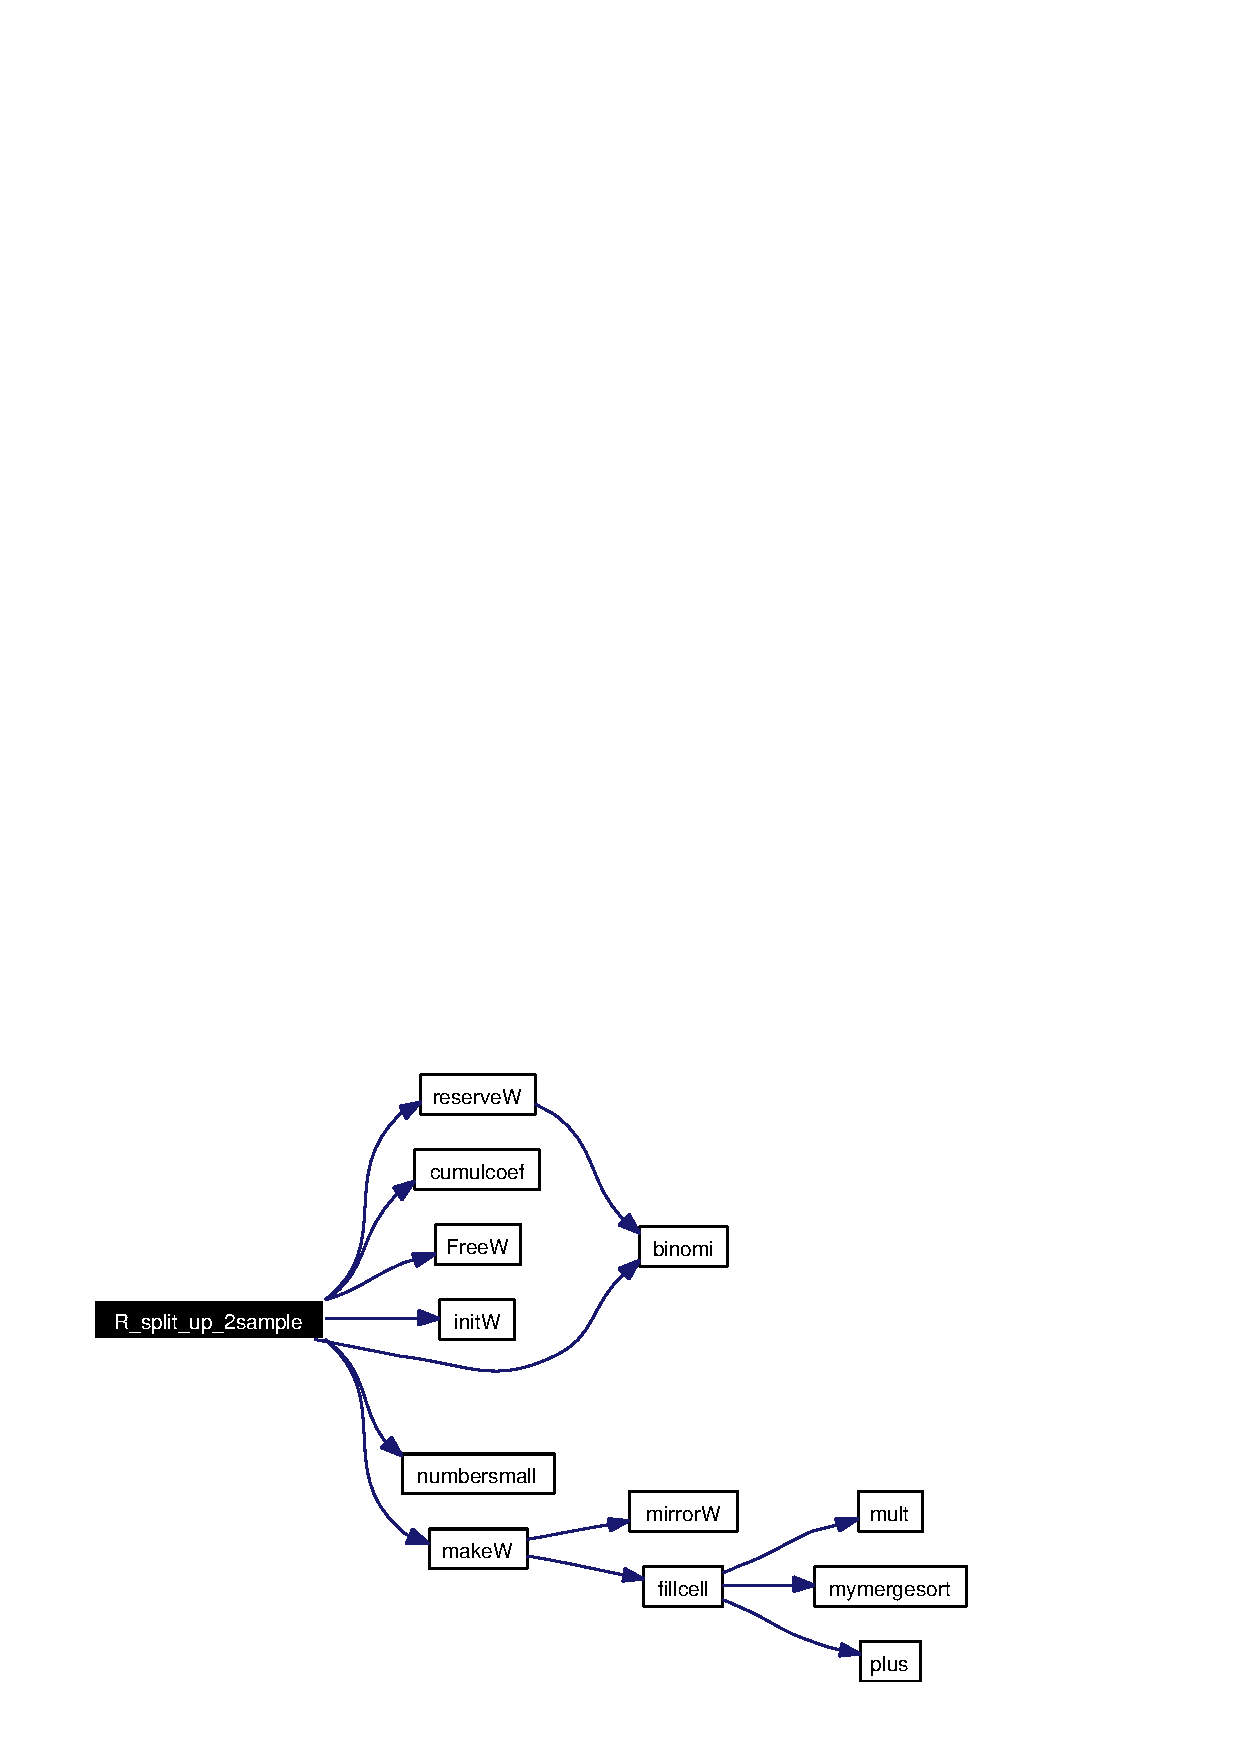
\includegraphics[width=227pt]{vandeWiel_8c_a12_cgraph}
\end{center}
\end{figure}
\hypertarget{vandeWiel_8c_a1}{
\index{vandeWiel.c@{vande\-Wiel.c}!reserveW@{reserveW}}
\index{reserveW@{reserveW}!vandeWiel.c@{vande\-Wiel.c}}
\subsubsection[reserveW]{\setlength{\rightskip}{0pt plus 5cm}\hyperlink{structcelW}{cel\-W}$\ast$$\ast$ reserve\-W (int {\em a}, int {\em b})}}
\label{vandeWiel_8c_a1}




Definition at line 51 of file vande\-Wiel.c.

References binomi(), cel\-W::c, and cel\-W::x.

Referenced by R\_\-split\_\-up\_\-2sample().

Here is the call graph for this function:\begin{figure}[H]
\begin{center}
\leavevmode
\includegraphics[width=89pt]{vandeWiel_8c_a1_cgraph}
\end{center}
\end{figure}

\hypertarget{vandeWiel_8d}{
\section{vande\-Wiel.d File Reference}
\label{vandeWiel_8d}\index{vandeWiel.d@{vandeWiel.d}}
}

\printindex
\end{document}
